\documentclass[12pt]{beamer}


%%%%% 26-02-2022 package multicol multirow
\newcommand{\mc}[2]{\multicolumn{#1}{c}{#2}}
\definecolor{Gray}{gray}{0.85}
\definecolor{LightCyan}{rgb}{0.88,1,1}
\usepackage{hhline,longtable}
\usepackage{tabularx,booktabs}

\usepackage{multicol}
\usepackage{multirow}
%% 26-02-2022
\usepackage{hhline,longtable}
\usepackage{threeparttable}

\usepackage{tabularx,booktabs}
\newcommand{\tabitem}{~~\llap{\textbullet}~~}


\usepackage{enumerate}
\usepackage[shortlabels]{enumitem}

\setlist[enumerate, 1]{label =\textbf{\arabic*.}}
\setlist[enumerate, 2]{label =\textbf{\theenumi \alph*}}
\usepackage{array,multirow}

\usepackage{amsmath,mathtools}

\usepackage{amssymb}
\usepackage{amsthm}
\usepackage{mathtools}



\DeclarePairedDelimiter\abs{\lvert}{\rvert}%
\DeclarePairedDelimiter\norm{\lVert}{\rVert}%

% Swap the definition of \abs* and \norm*, so that \abs
% and \norm resizes the size of the brackets, and the 
% starred version does not.
\makeatletter
\let\oldabs\abs
\def\abs{\@ifstar{\oldabs}{\oldabs*}}










%%%% animation package 21-09-2021
\usepackage{animate}


%%%%%%%%%%%%%%%%%09-09-2021\\\ copied from Webinarinnovation page
% Here I would like to make a new command to change the transparency of a photo and put it as a background photo
\usepackage{tikz}



%%%%%%%%%%%% 22-10-2020 Background block package
% beamer: How to place images behind text (z-order)
% (http://tex.stackexchange.com/a/134311)
\makeatletter
\newbox\@backgroundblock
\newenvironment{backgroundblock}[2]{%
  \global\setbox\@backgroundblock=\vbox\bgroup%
    \unvbox\@backgroundblock%
    \vbox to0pt\bgroup\vskip#2\hbox to0pt\bgroup\hskip#1\relax%
}{\egroup\egroup\egroup}
\addtobeamertemplate{background}{\box\@backgroundblock}{}
\makeatother

%%%%%%%%%%%%%%%%%%%%%%%%%%%%%%%%%%%%%%%%%%%%
%%%%%%%%%%%26-10-2020% set figure number
\setbeamertemplate{caption}[numbered]


%%%%%%%%%%%%%%%%26-10-2020
\usepackage{amssymb,amsmath}


%%%%%%%%%%%%%%%%26-10-2020
\newenvironment{variableblock}[3]{%
  \setbeamercolor{block body}{#2}
  \setbeamercolor{block title}{#3}
  \begin{block}{#1}}{\end{block}}
  
  \setbeamercolor{block body alerted}{bg=alerted text.fg!10}
\setbeamercolor{block title alerted}{bg=alerted text.fg!20}
\setbeamercolor{block body}{bg=structure!10}
\setbeamercolor{block title}{bg=structure!20}
\setbeamercolor{block body example}{bg=green!10}
\setbeamercolor{block title example}{bg=green!20}

\setbeamertemplate{blocks}[rounded][shadow=true]


%%%%%%%%%%%%%%%%%%%%%26-10-2020
\setbeamertemplate{footline}[frame number]

%%%%%%%%%%%% 26-10-2020
\usepackage{color, colortbl}
\definecolor{Gray}{gray}{0.85}

%%%%%%%%%%%%%%%%%%27-10-2020
\usepackage[T1]{fontenc}



\title{\large \textbf{Large-Scale Integration of EVs, one Application of the High-Performace Solver: BATTPOWER}}
\begin{backgroundblock}{20mm}{20mm}
    \begin{tikzpicture}
    \node[anchor=east,inner sep=0] (B) at (4,0) {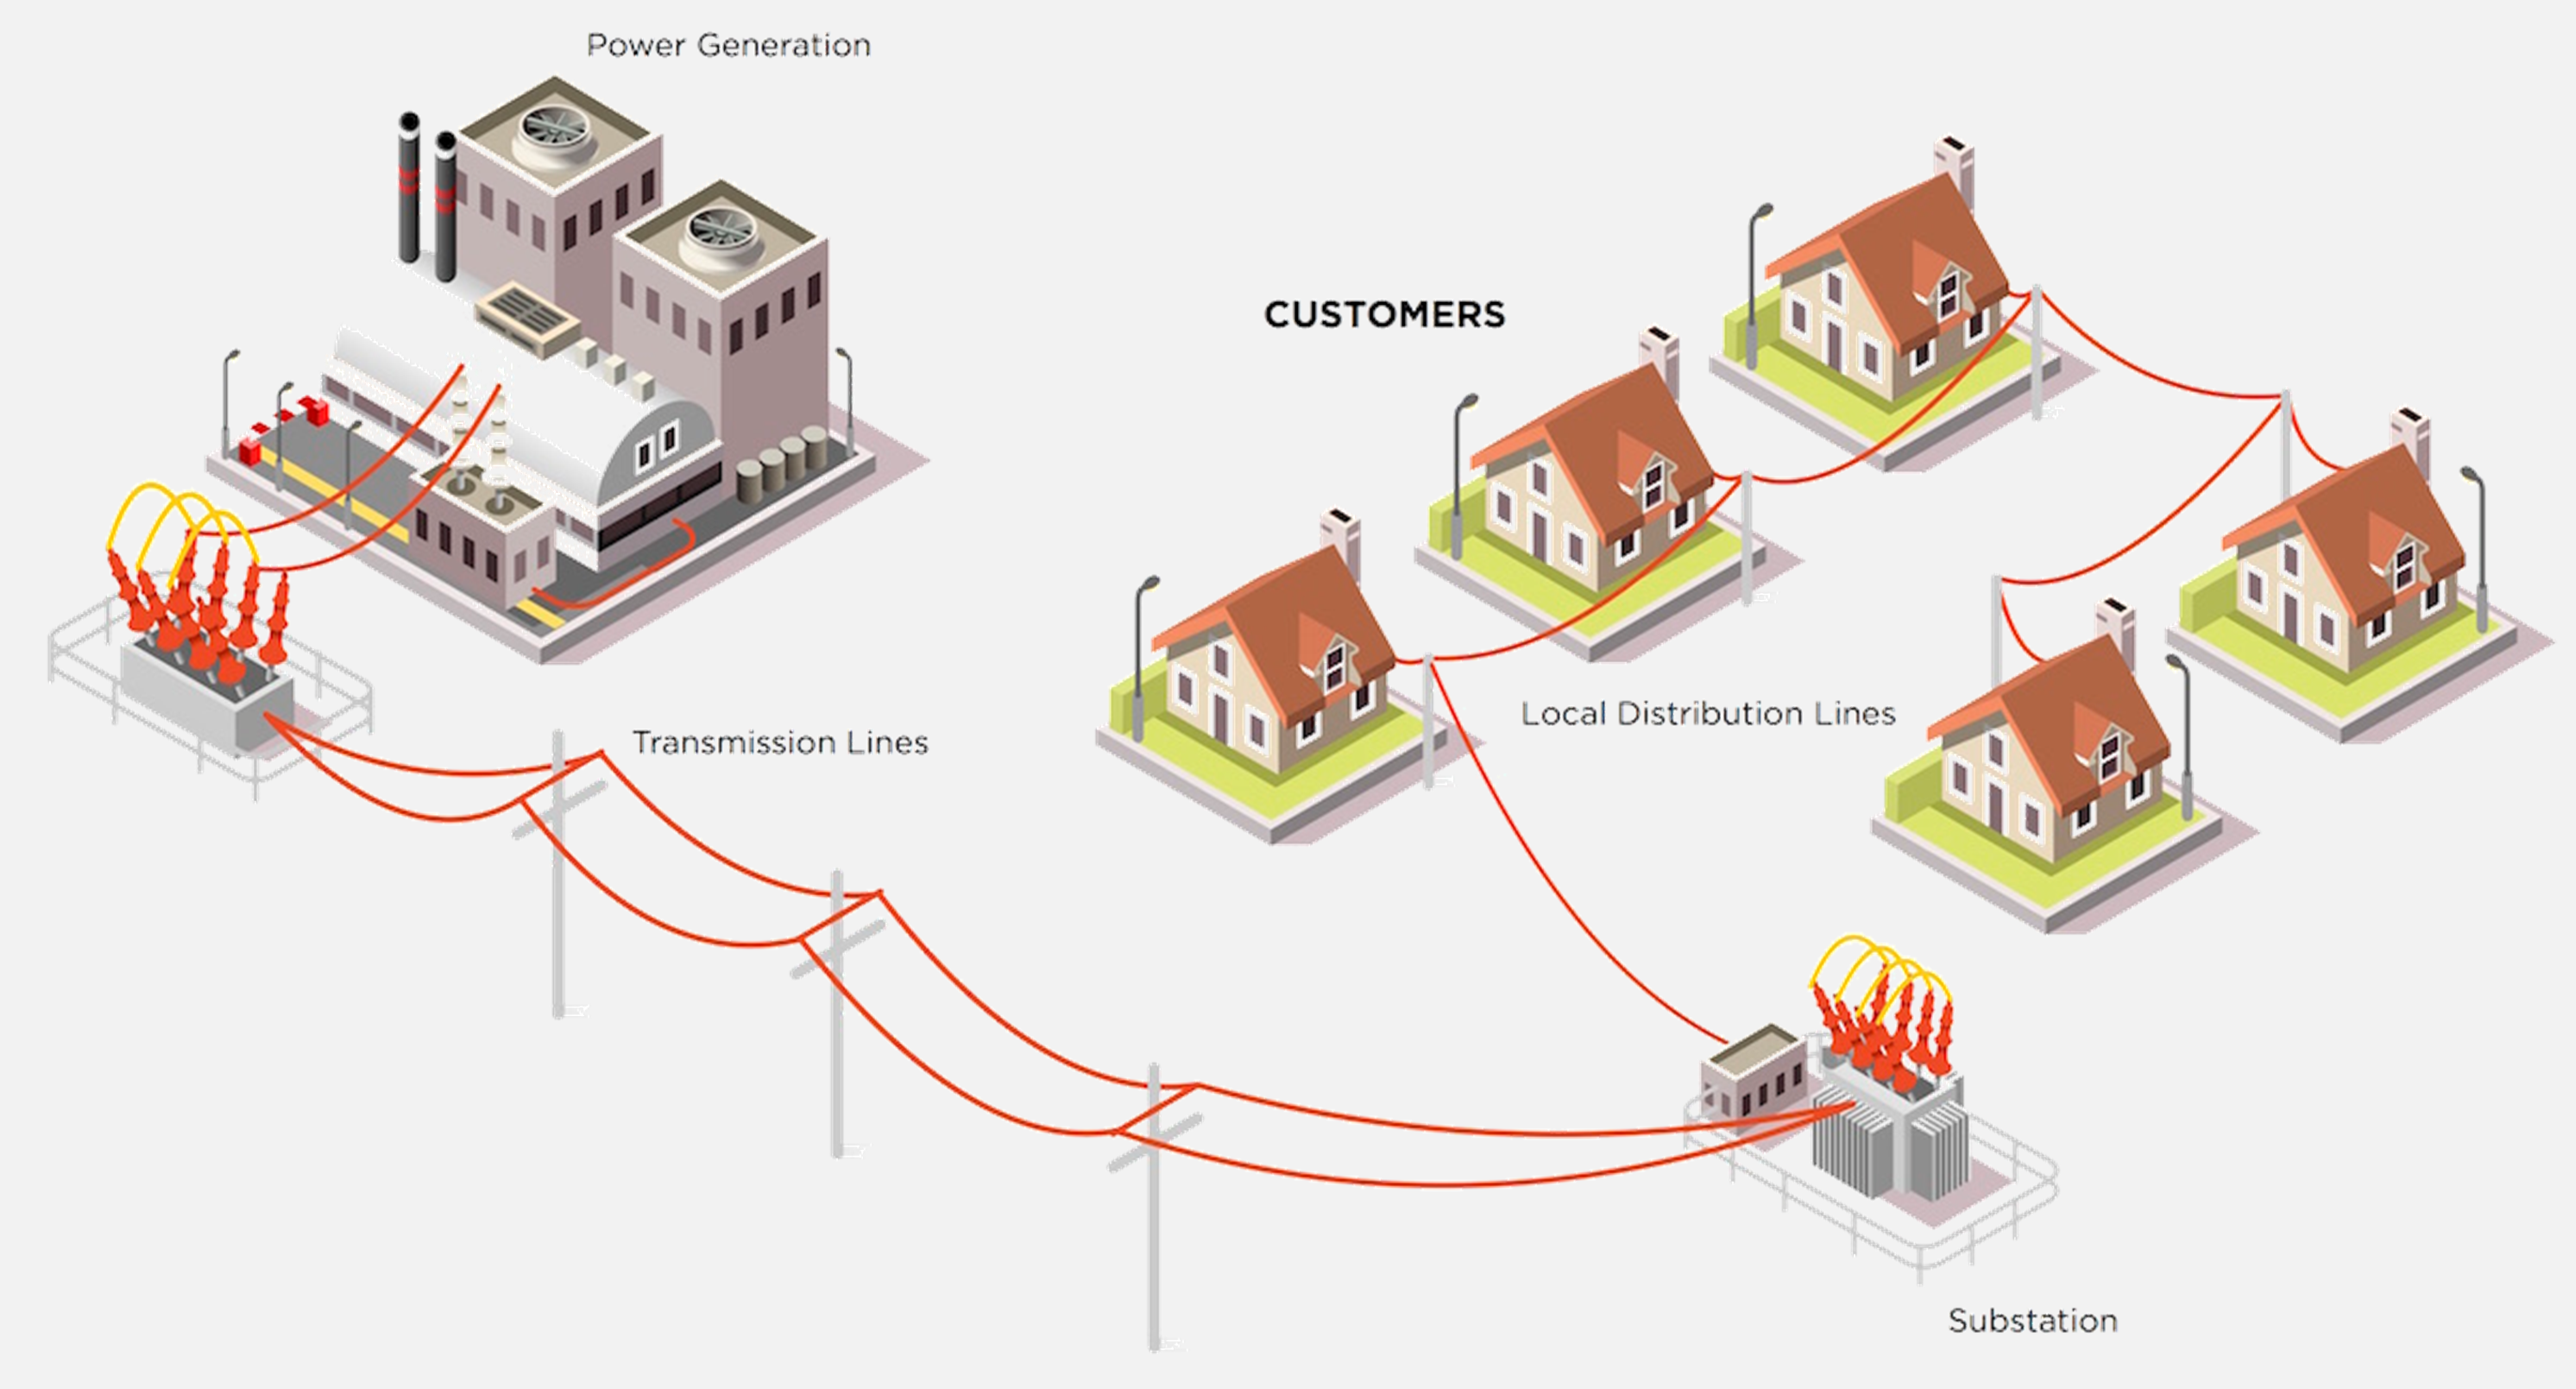
\includegraphics[width=\linewidth]{Figures/PowerSys.png}};
           \fill [draw=none, fill=white, fill opacity=0.7] (B.north west) -- (B.north east) -- (B.south east) -- (B.south west) -- (B.north west) -- cycle;
 
    \end{tikzpicture} 
    \end{backgroundblock} 

\logo{%
    
\includegraphics[width=3cm,height=3cm,keepaspectratio]{ntnulogo_eng}~%
}


\author{Salman Zaferanlouei}
\institute{NTNU{\\ \vskip 1cm} \scalebox{1.5}{\insertlogo}}
\date{\today}









\begin{document}
\begin{frame}
\titlepage
\end{frame}
%%%%%%%%%%%%%%%%%%%%%%%%%%%%%%%%%%%%%%%%%%
%%%%%%%%%%%%%%%%%%%%%%%%%%%%%%%%%%%%%%%%%%
%%%%%%%%%%%%%%%%%%%%%%%%%%%%%%%%%%%%%%%%%%
%%%%%%%%%%%%%%%%%%%%%%%%%%%%%%%%%%%%%%%%%%




%%%%%%%%%%%%%%%%%%%%%%%%%%%%%%%%%%%%%%%%%%
%%%%%%%%%%%%%%%%%%%%%%%%%%%%%%%%%%%%%%%%%%
%%%%%%%%%%%%%%%%%%%%%%%%%%%%%%%%%%%%%%%%%%
%%%%%%%%%%%%%%%%%%%%%%%%%%%%%%%%%%%%%%%%%%

\begin{frame}{Purpose}
\begin{itemize}
\item \textbf{Purpose:} To share my  experiences from Research to Innovation. 
\item \textbf{Time}: 20 min
\item \textbf{Target:} NTNU Employees and Students
\end{itemize}
\begin{center}
\begin{tabular}{|l l|} 
\hline
\rowcolor{Gray} \textbf{Project Name:} &Battpower \\
\textbf{Time Spent:}& Five Years\\
\hline
\end{tabular}
\end{center}
\end{frame}

%%%%%%%%%%%%%%%%%%%%%%%%%%%%%%%%%%%%%%%%%%
%%%%%%%%%%%%%%%%%%%%%%%%%%%%%%%%%%%%%%%%%%
%%%%%%%%%%%%%%%%%%%%%%%%%%%%%%%%%%%%%%%%%%
%%%%%%%%%%%%%%%%%%%%%%%%%%%%%%%%%%%%%%%%%%
\section{My Idea}
\begin{frame}{Idea}

 \begin{columns}
    \column{0.85\textwidth}
    \only<1>{
\begin{figure}[!htbp]
\centering
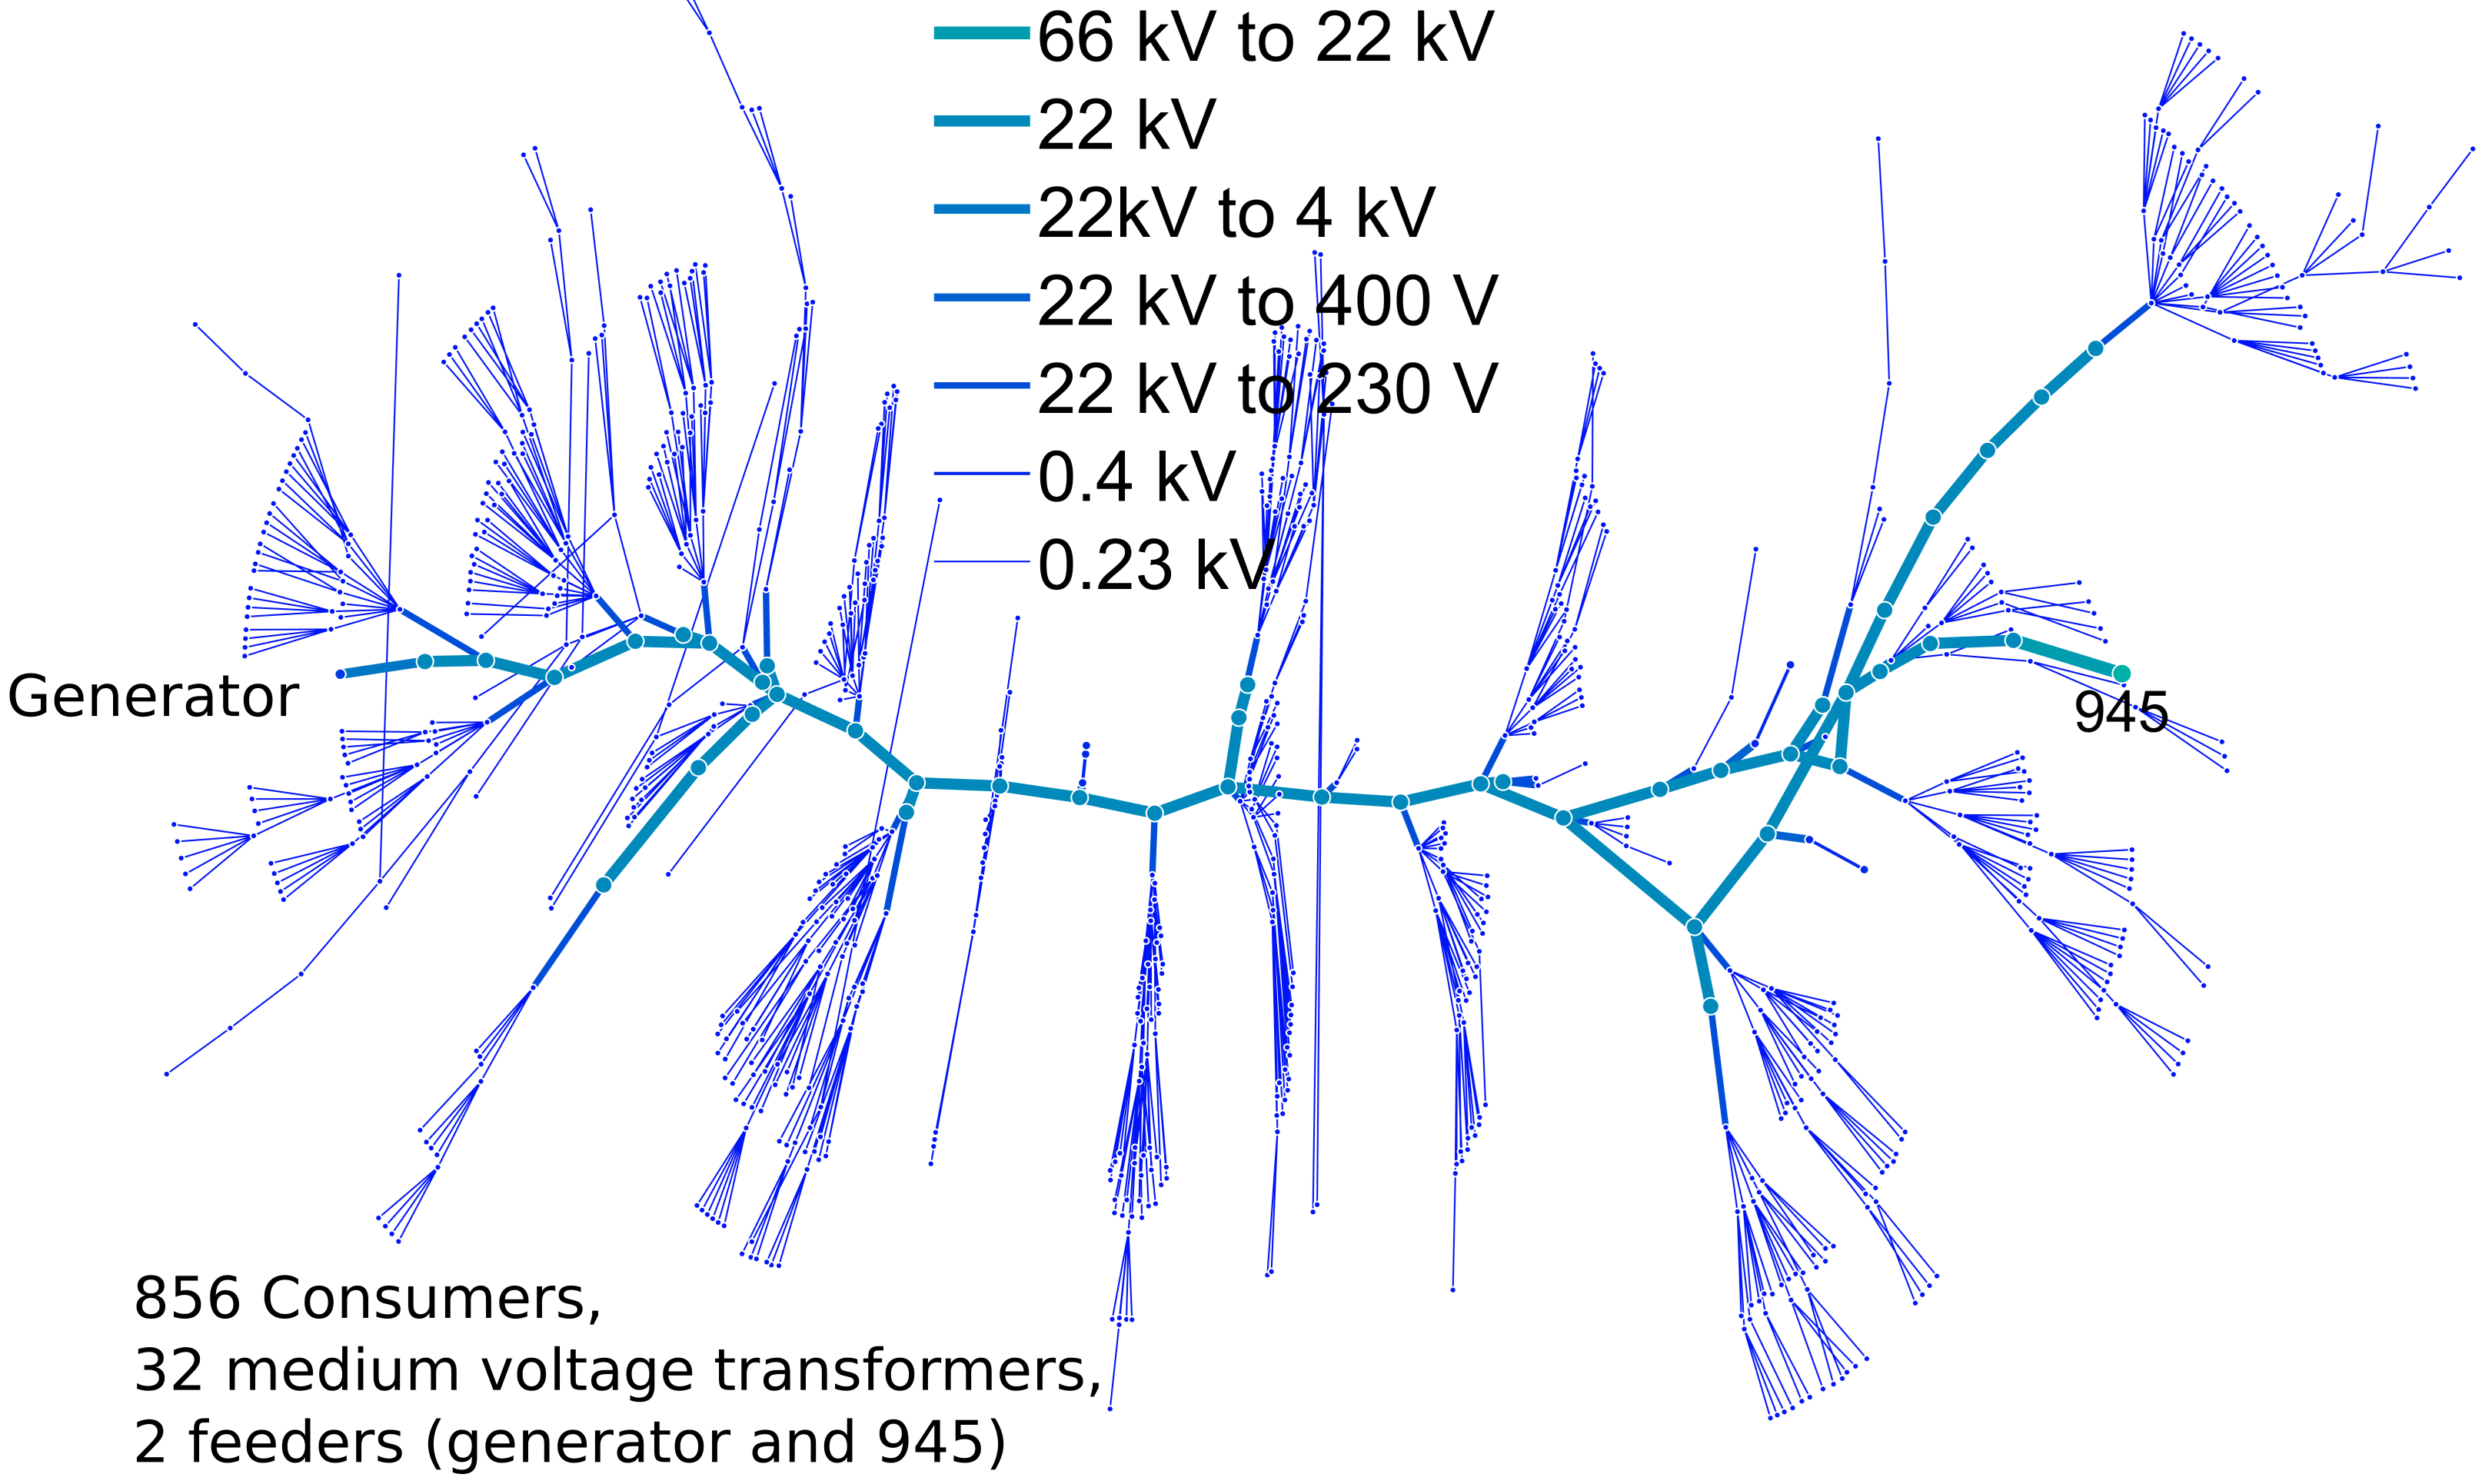
\includegraphics[width=3.3 in , height=2 in]{Figures/DistributionGridmodified.png}
\caption{Local distribution grid located in Norway with 856 costumers}
\label{Norwegian1}
\end{figure}}
\only<2>{
\begin{figure}[!htbp]
\centering
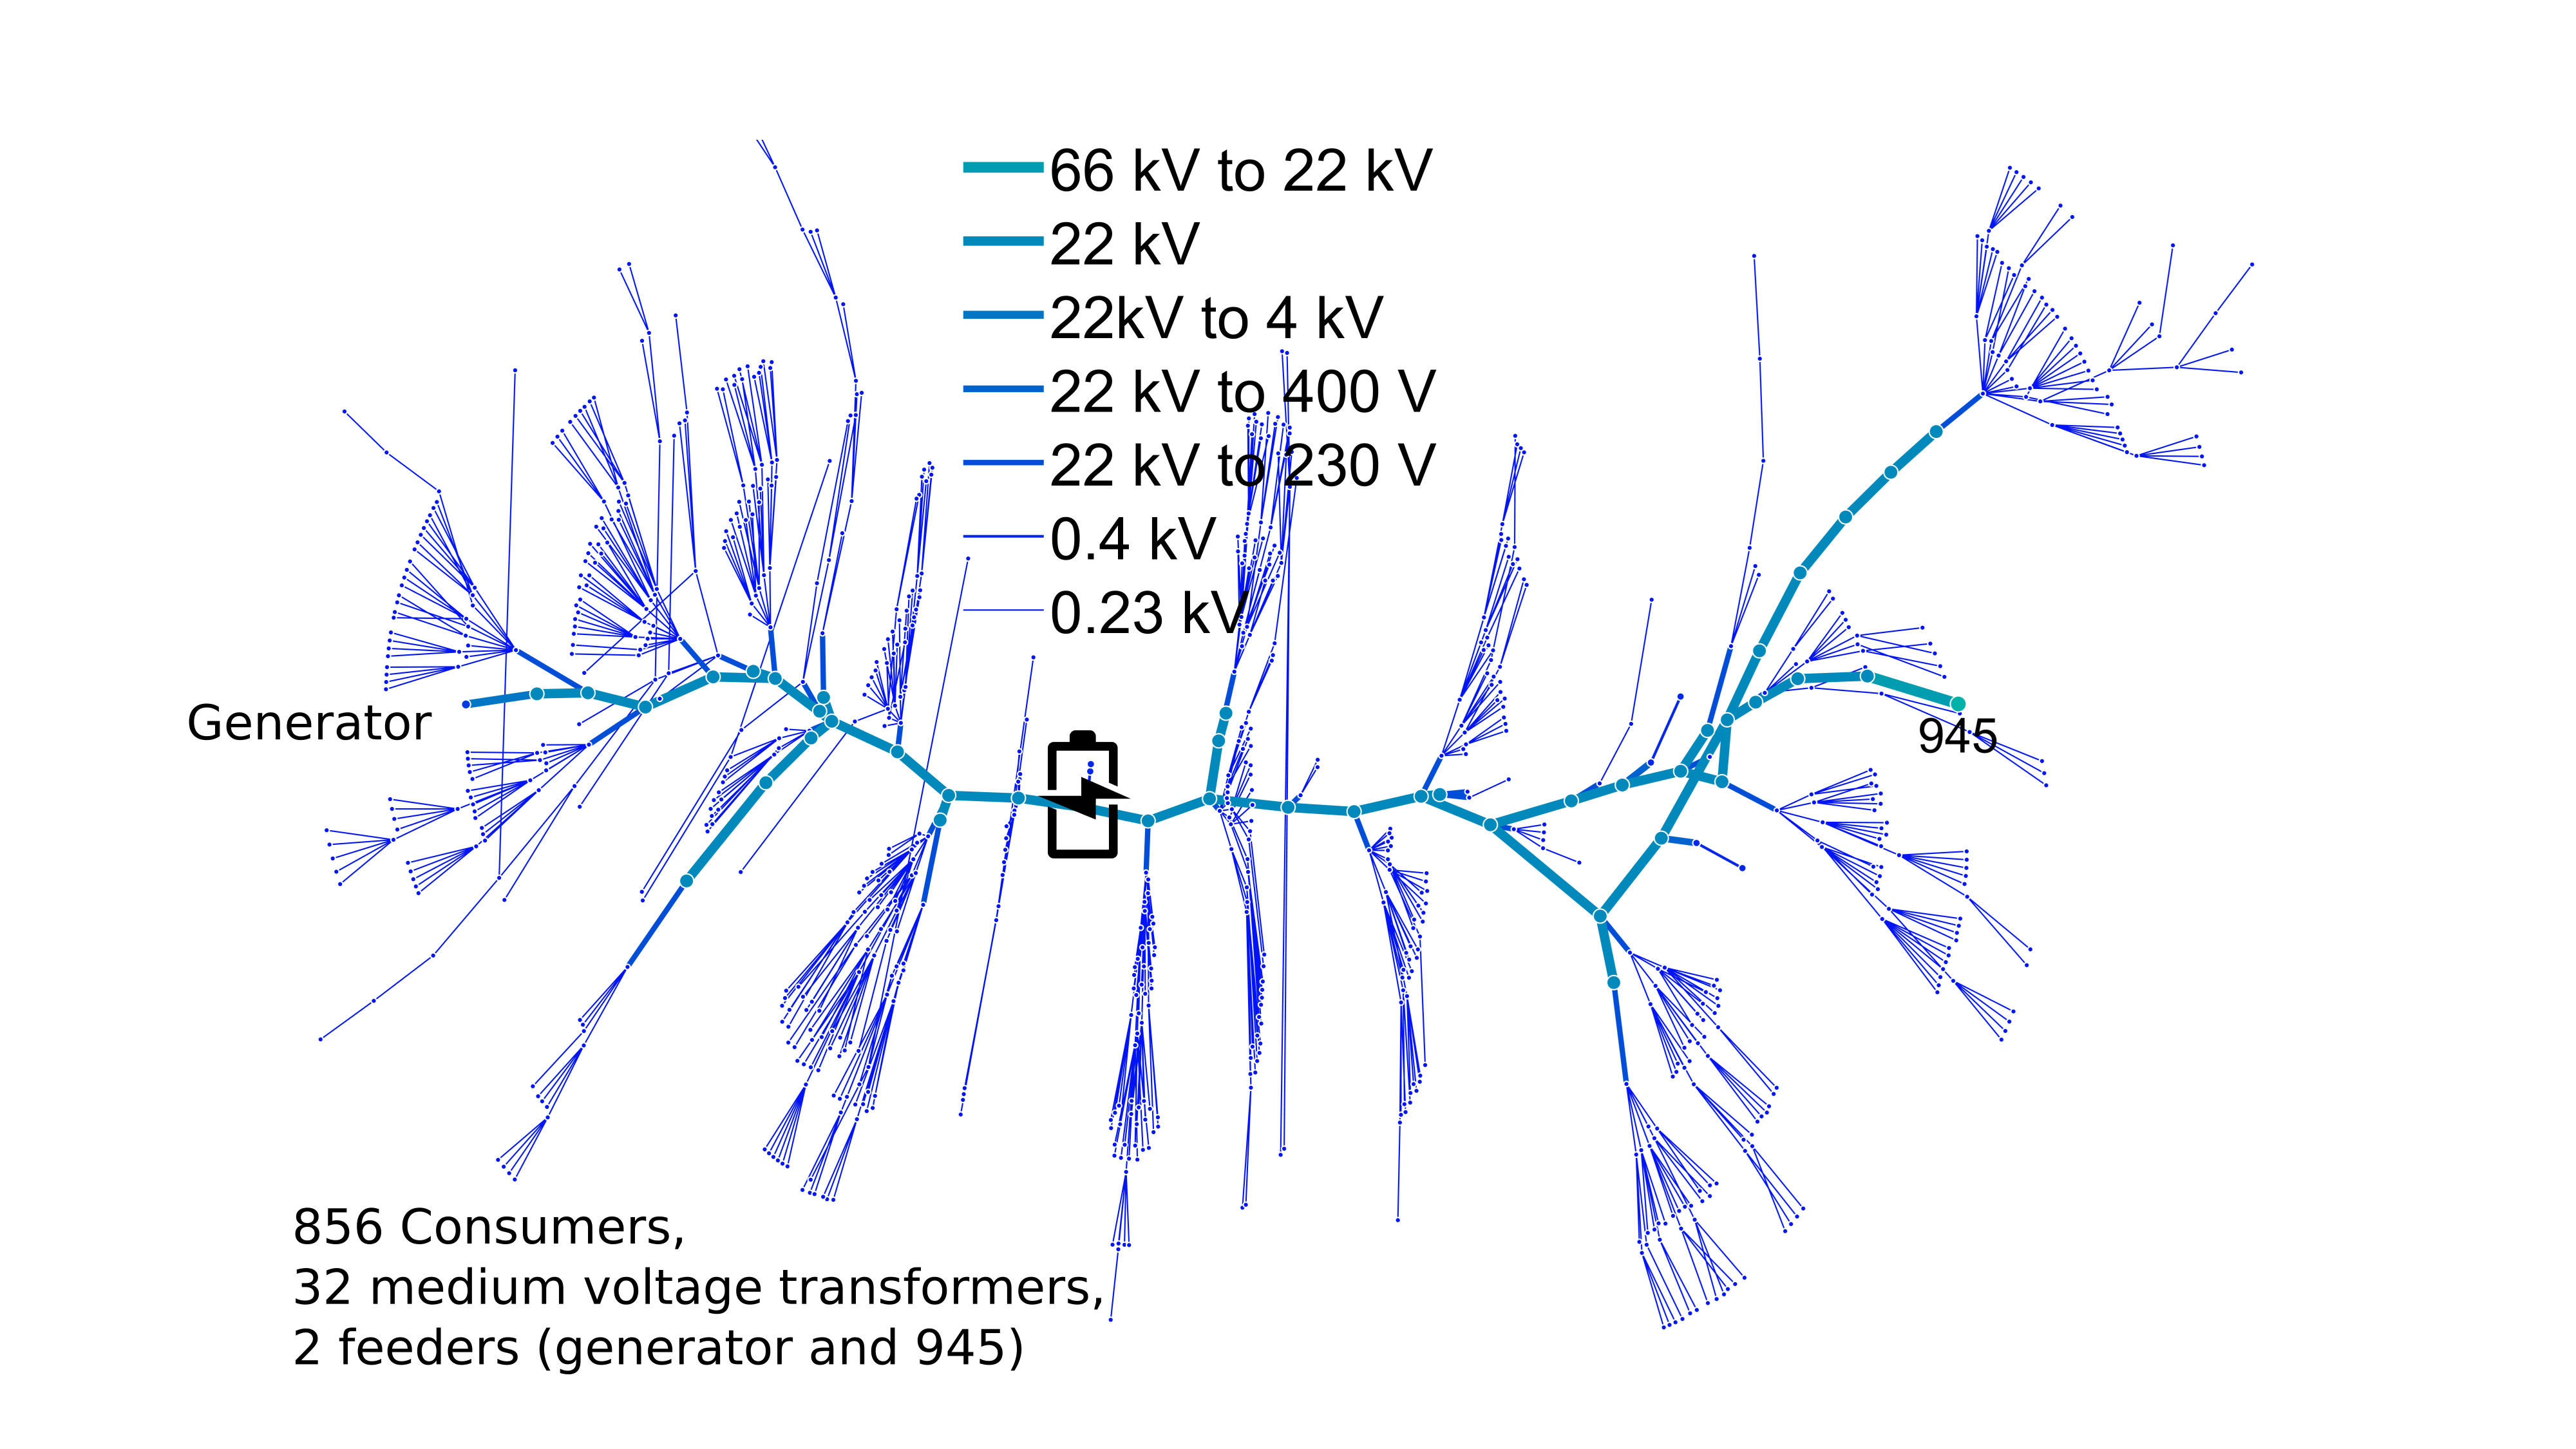
\includegraphics[width=3.5 in , height=2 in]{Figures/Presentation1/Slide1.png}
\caption{Local distribution grid located in Norway with 856 costumers}
\label{Norwegian1}
\end{figure}}
\only<3>{
\begin{figure}[!htbp]
\centering
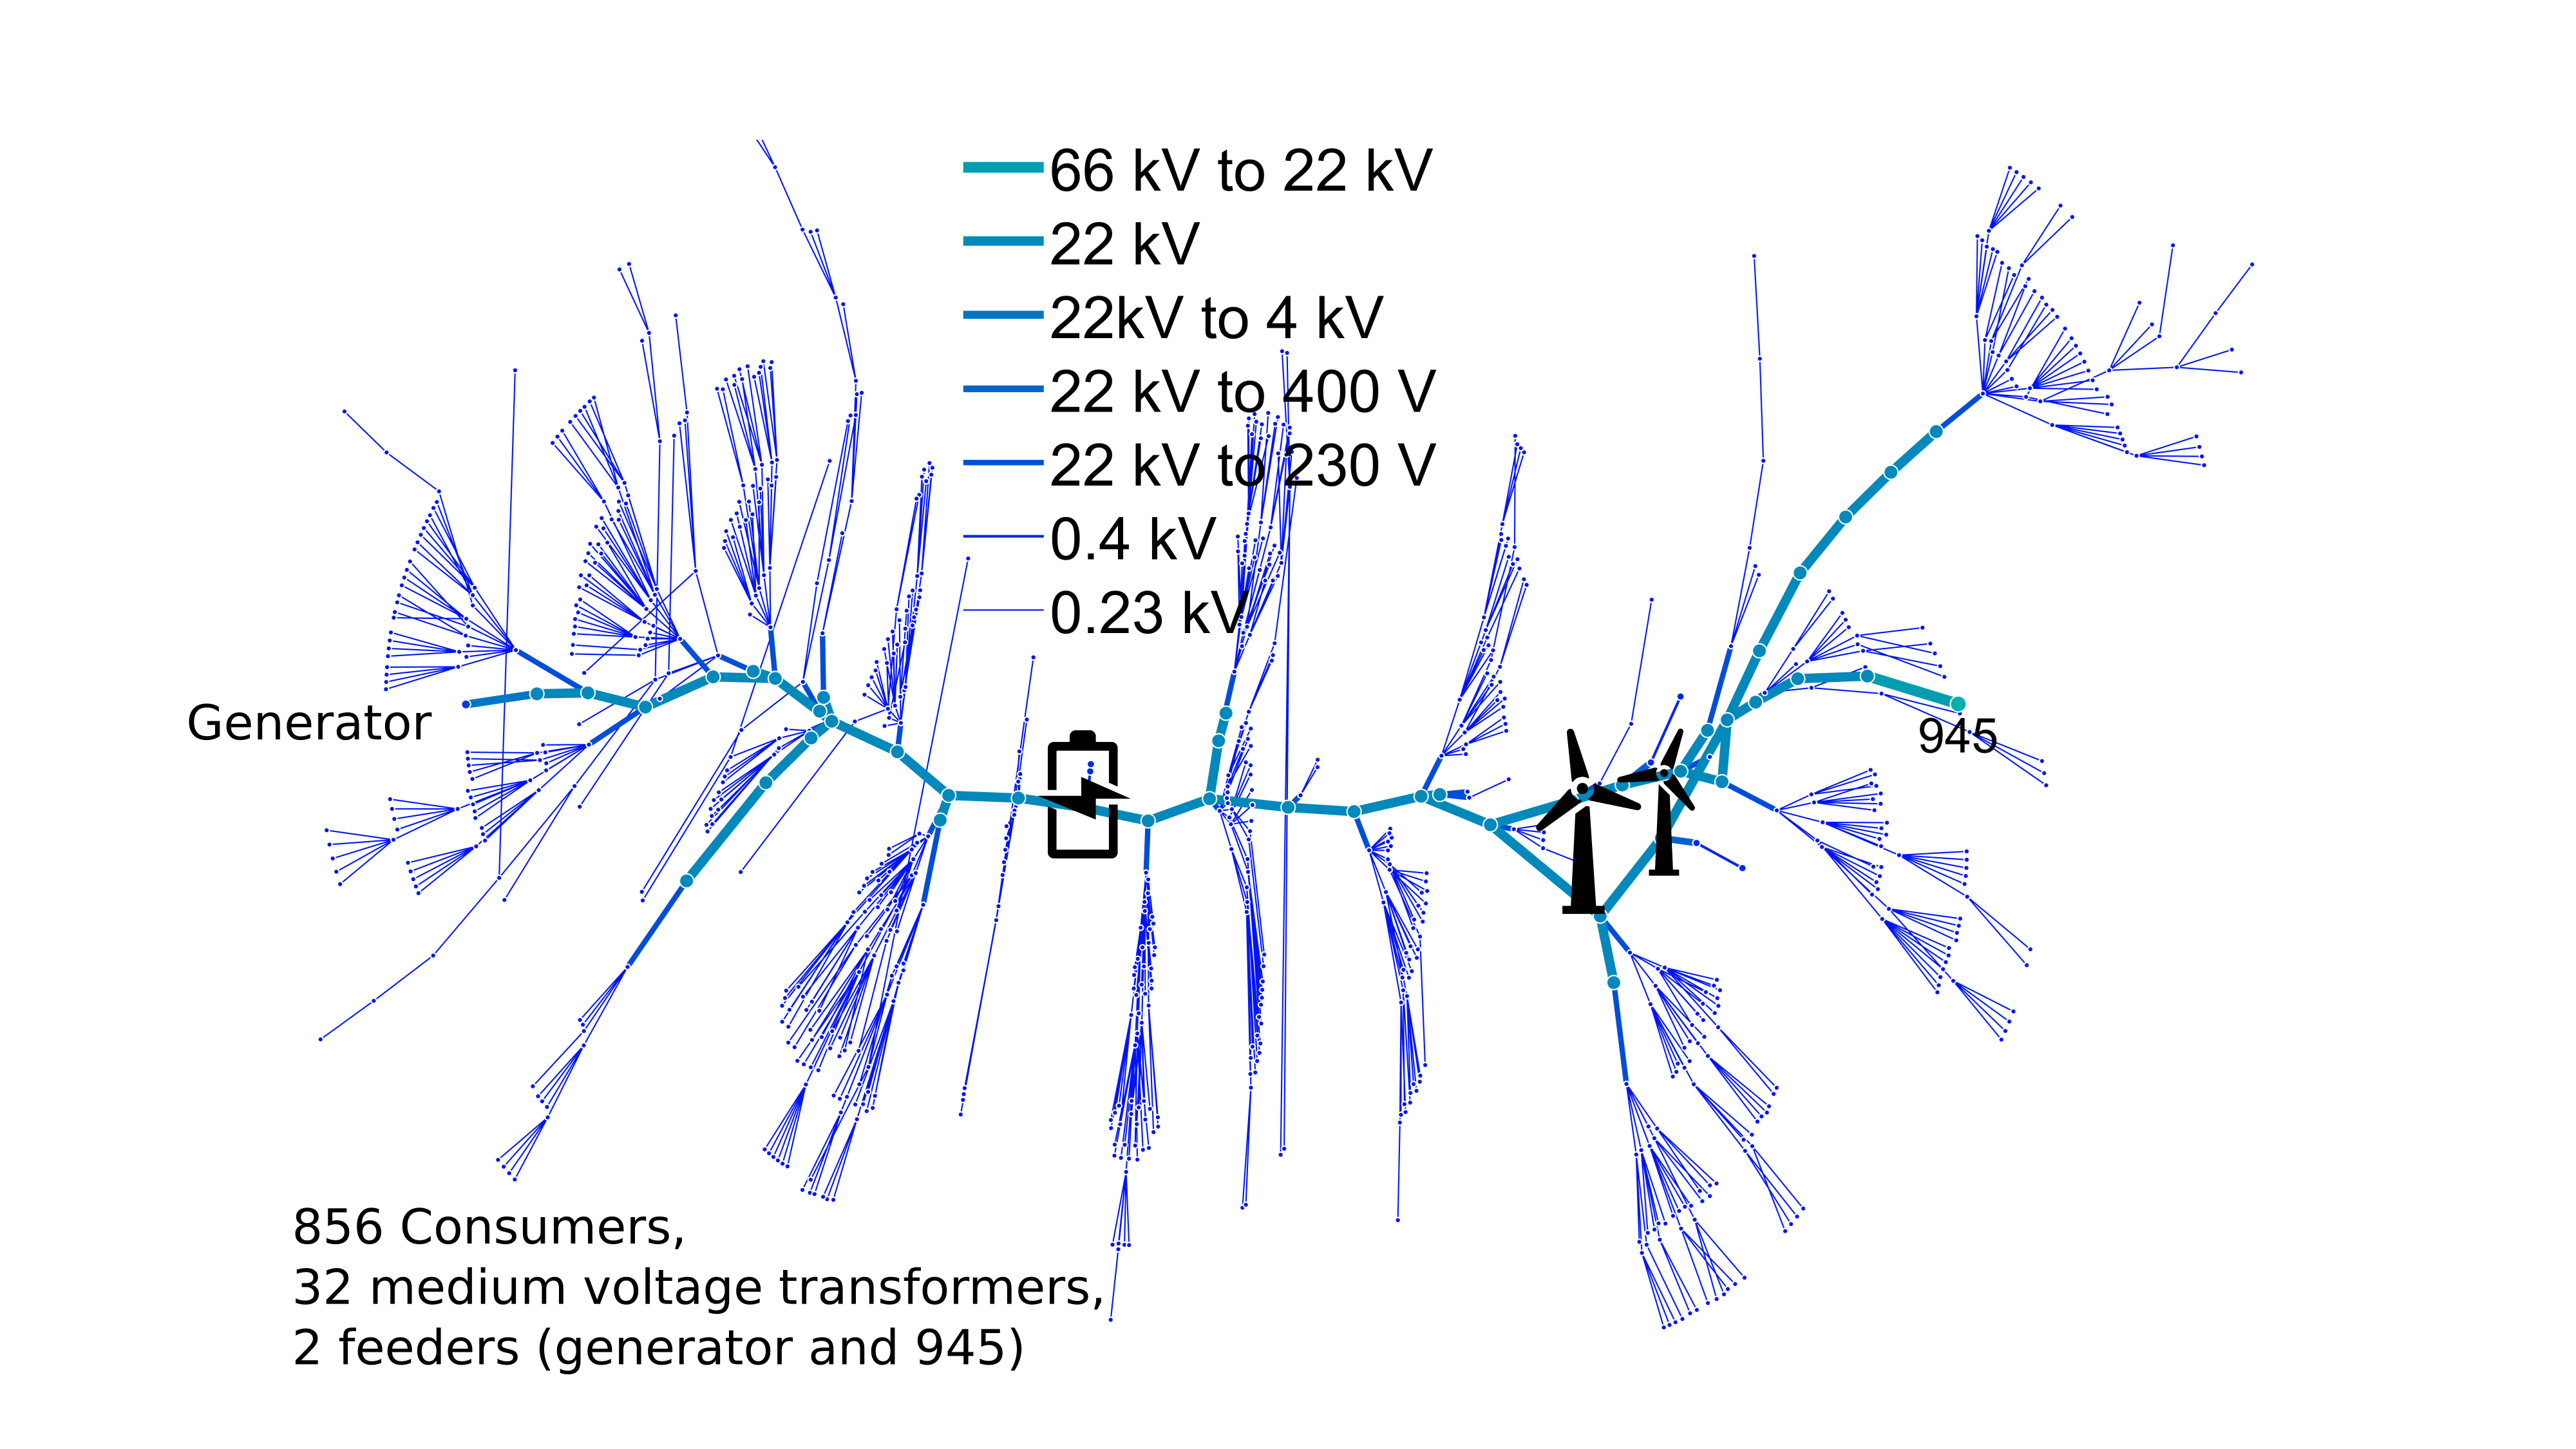
\includegraphics[width=3.5 in , height=2 in]{Figures/Presentation1/Slide2.png}
\caption{Local distribution grid located in Norway with 856 costumers}
\label{Norwegian1}
\end{figure}}
\only<4>{
\begin{figure}[!htbp]
\centering
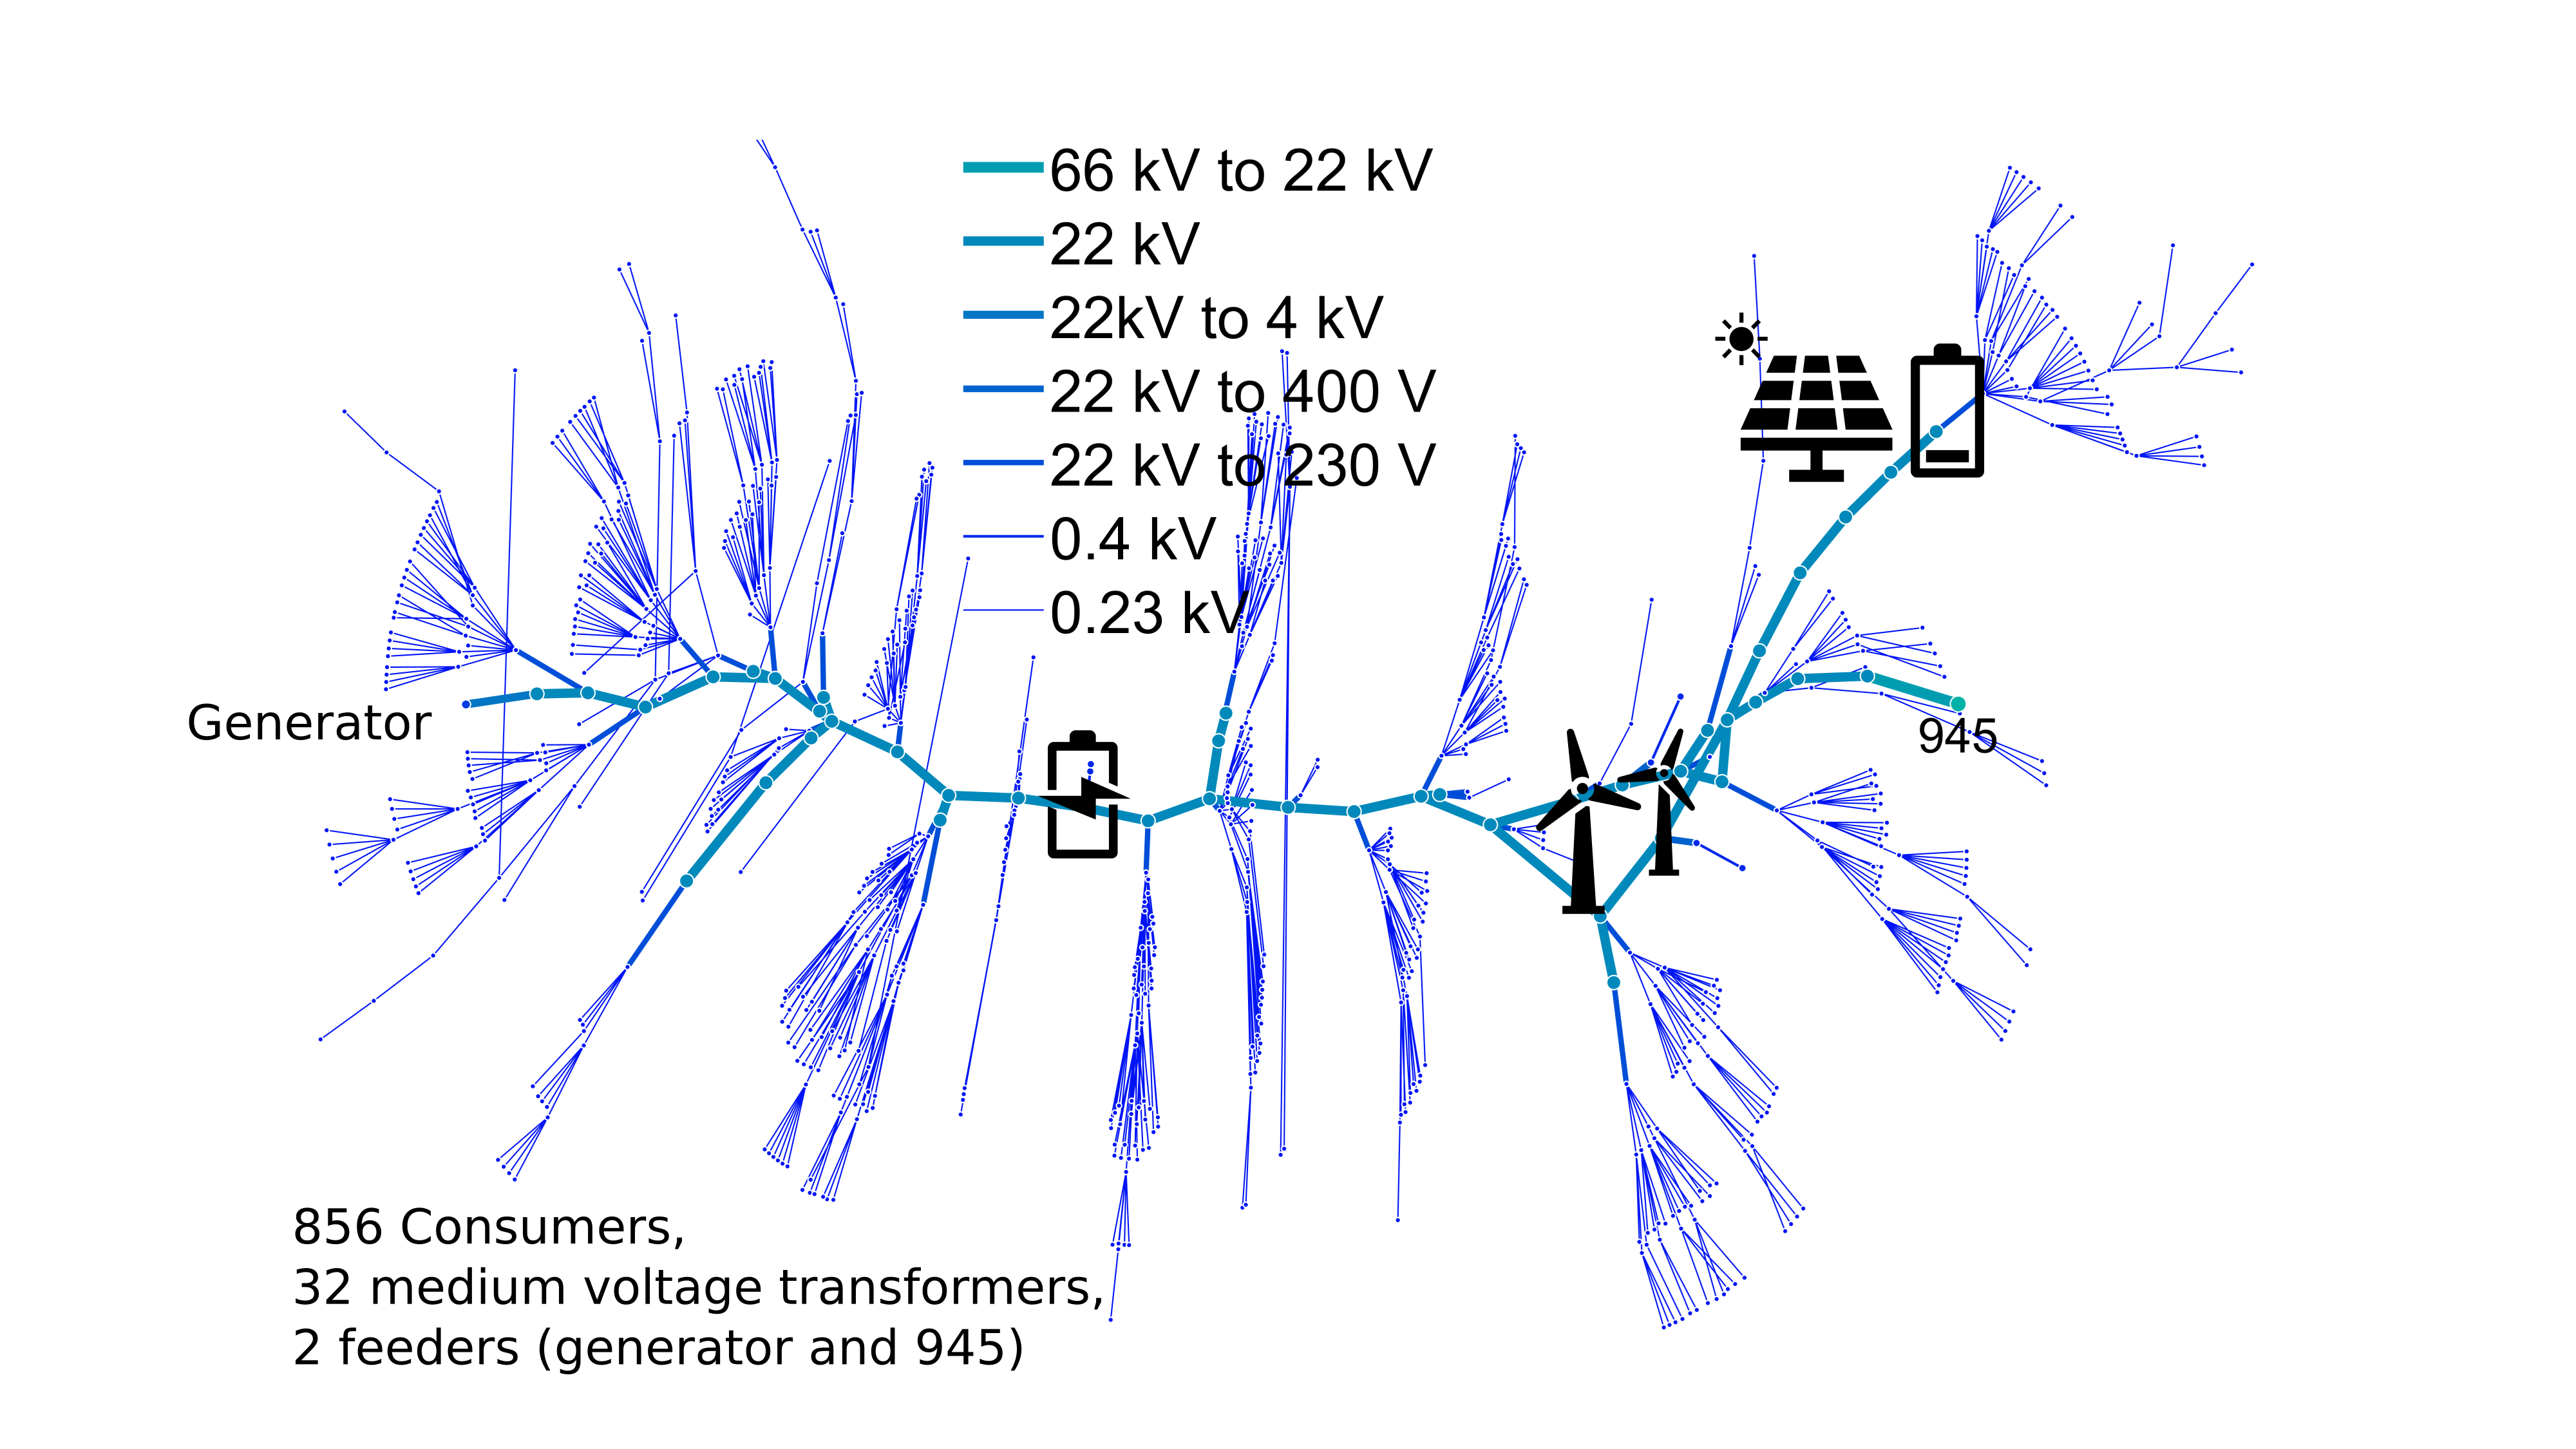
\includegraphics[width=3.5 in , height=2 in]{Figures/Presentation1/Slide3.png}
\caption{Local distribution grid located in Norway with 856 costumers}
\label{Norwegian1}
\end{figure}}
\only<5>{
\begin{figure}[!htbp]
\centering
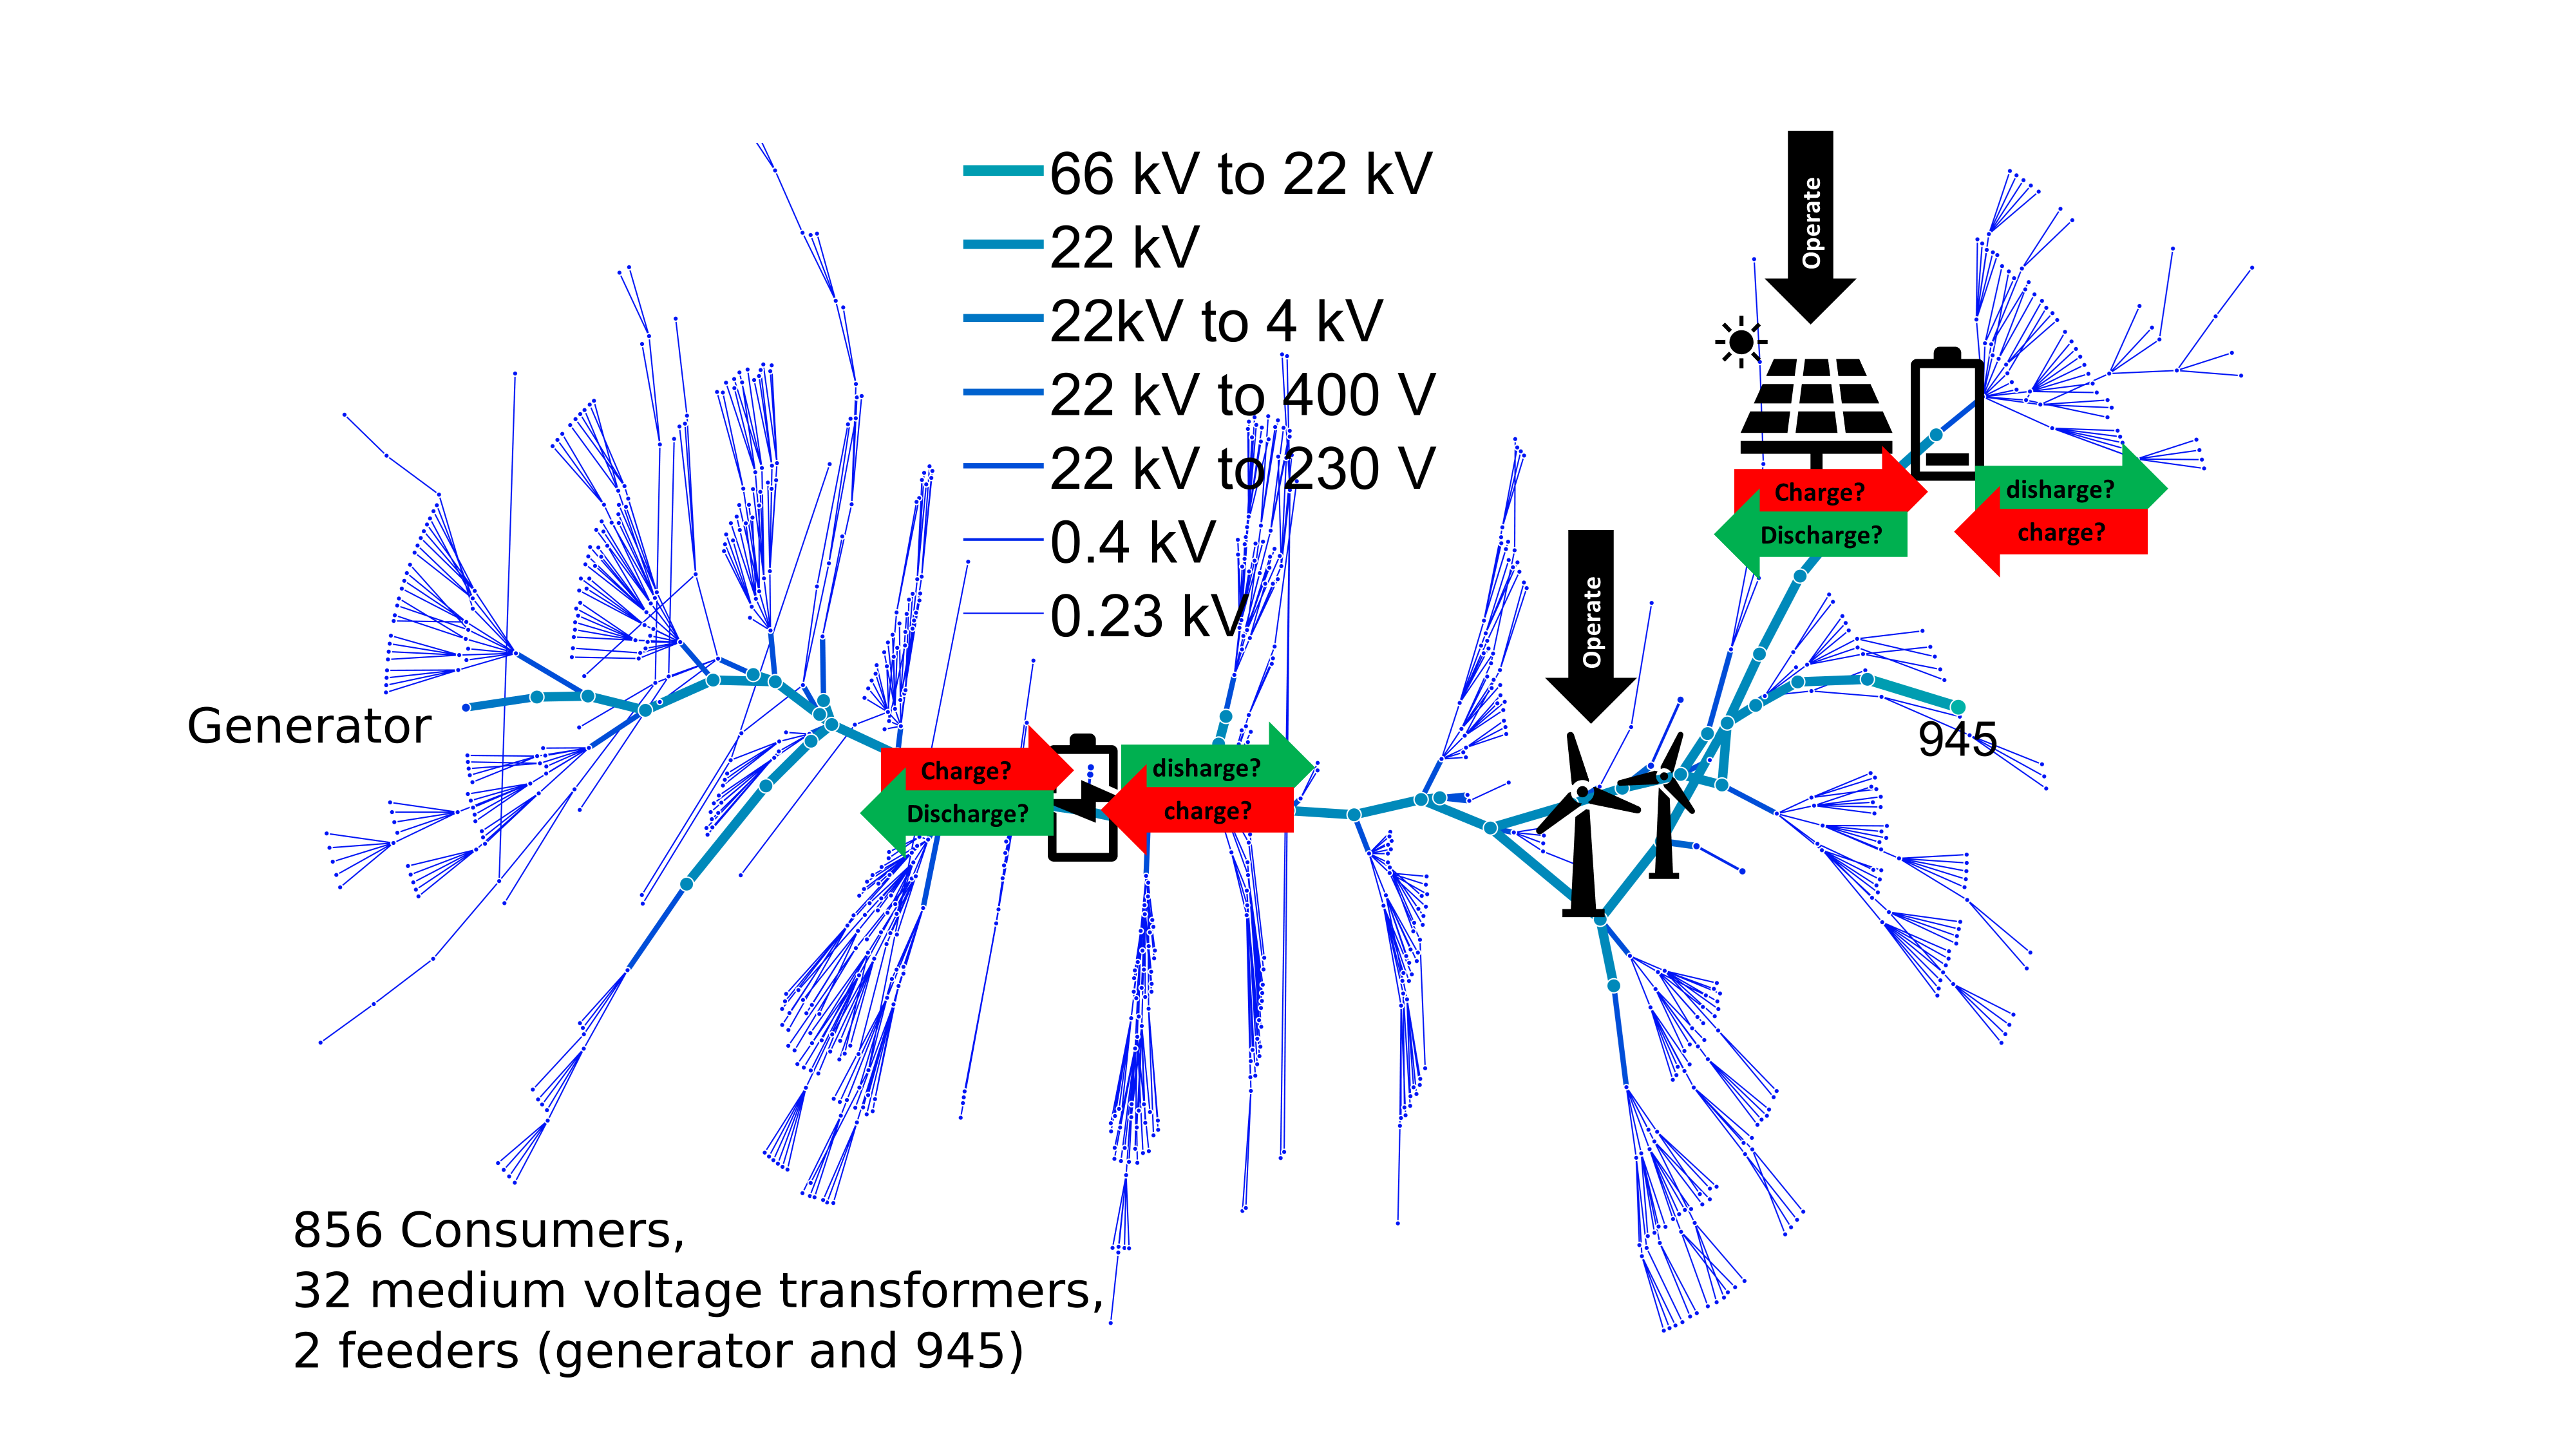
\includegraphics[width=3.5 in , height=2 in]{Figures/Presentation2/Slide1.png}
\caption{Local distribution grid located in Norway with 856 costumers}
\label{Norwegian1}
\end{figure}}
\only<6>{
\begin{figure}[!htbp]
\centering
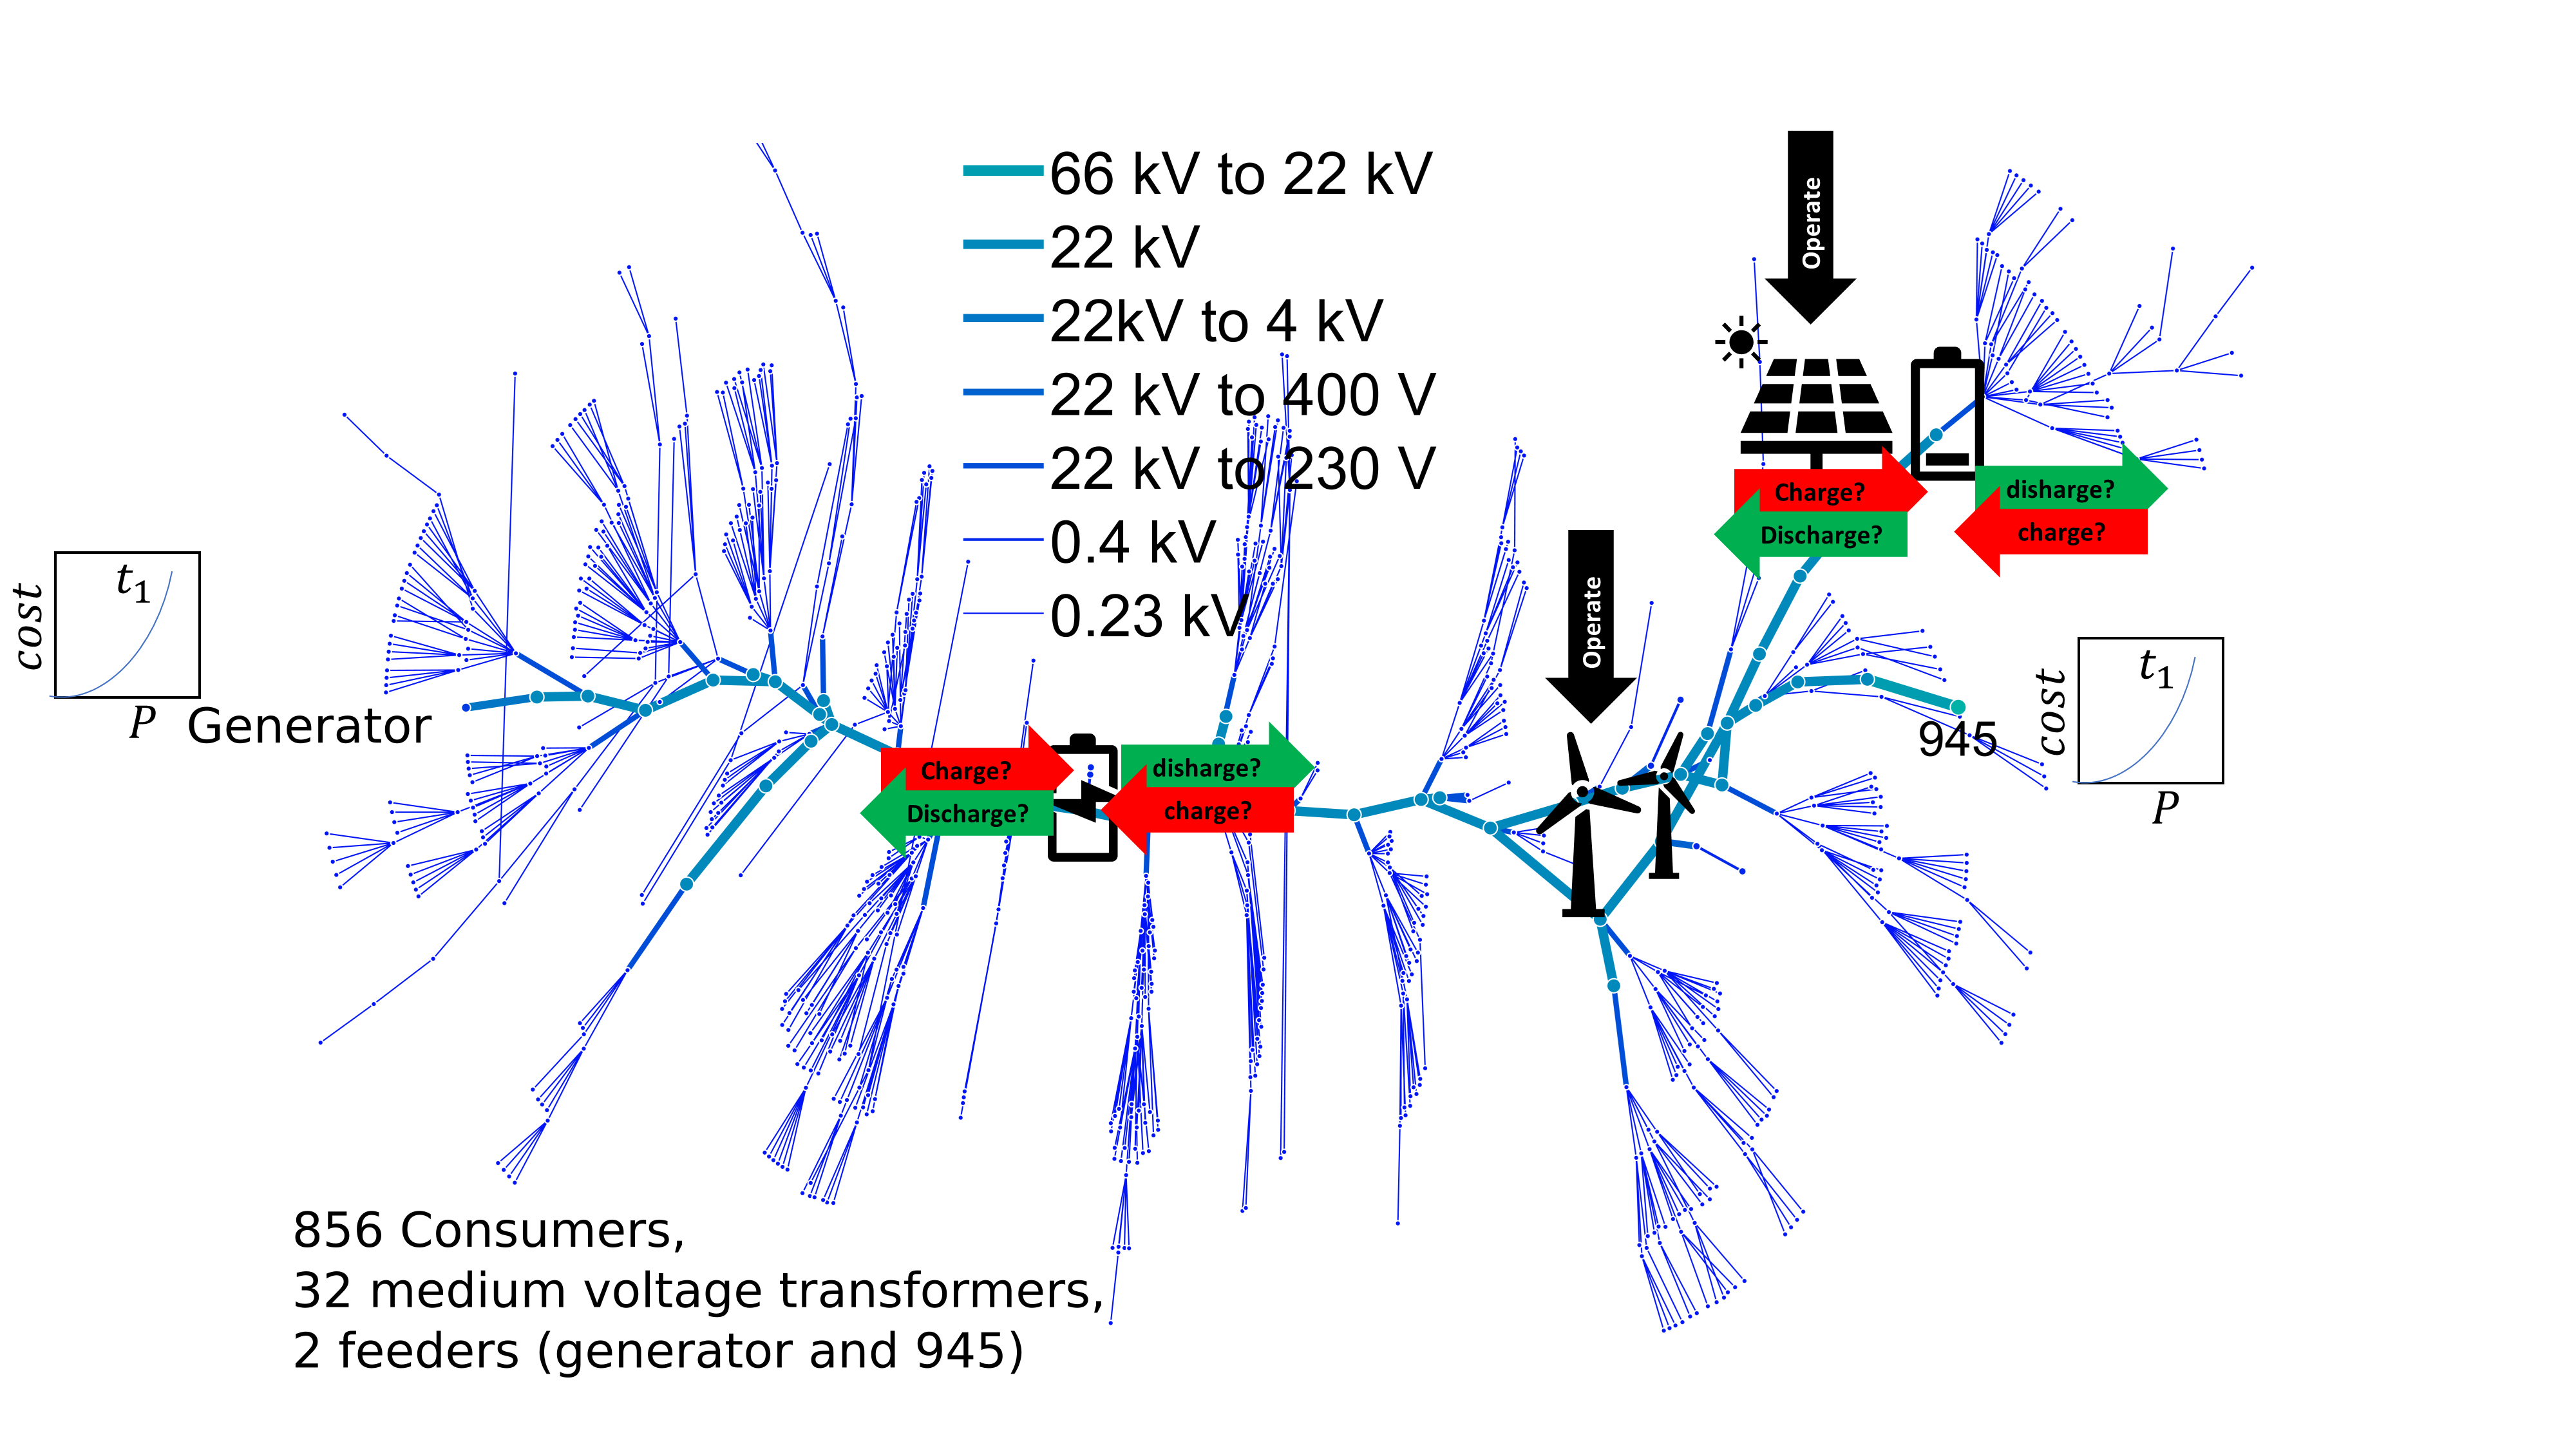
\includegraphics[width=3.5 in , height=2 in]{Figures/Presentation2/Slide2.png}
\caption{Local distribution grid located in Norway with 856 costumers}
\label{Norwegian1}
\end{figure}}
     
\only<7>{
\begin{figure}[!htbp]
\centering
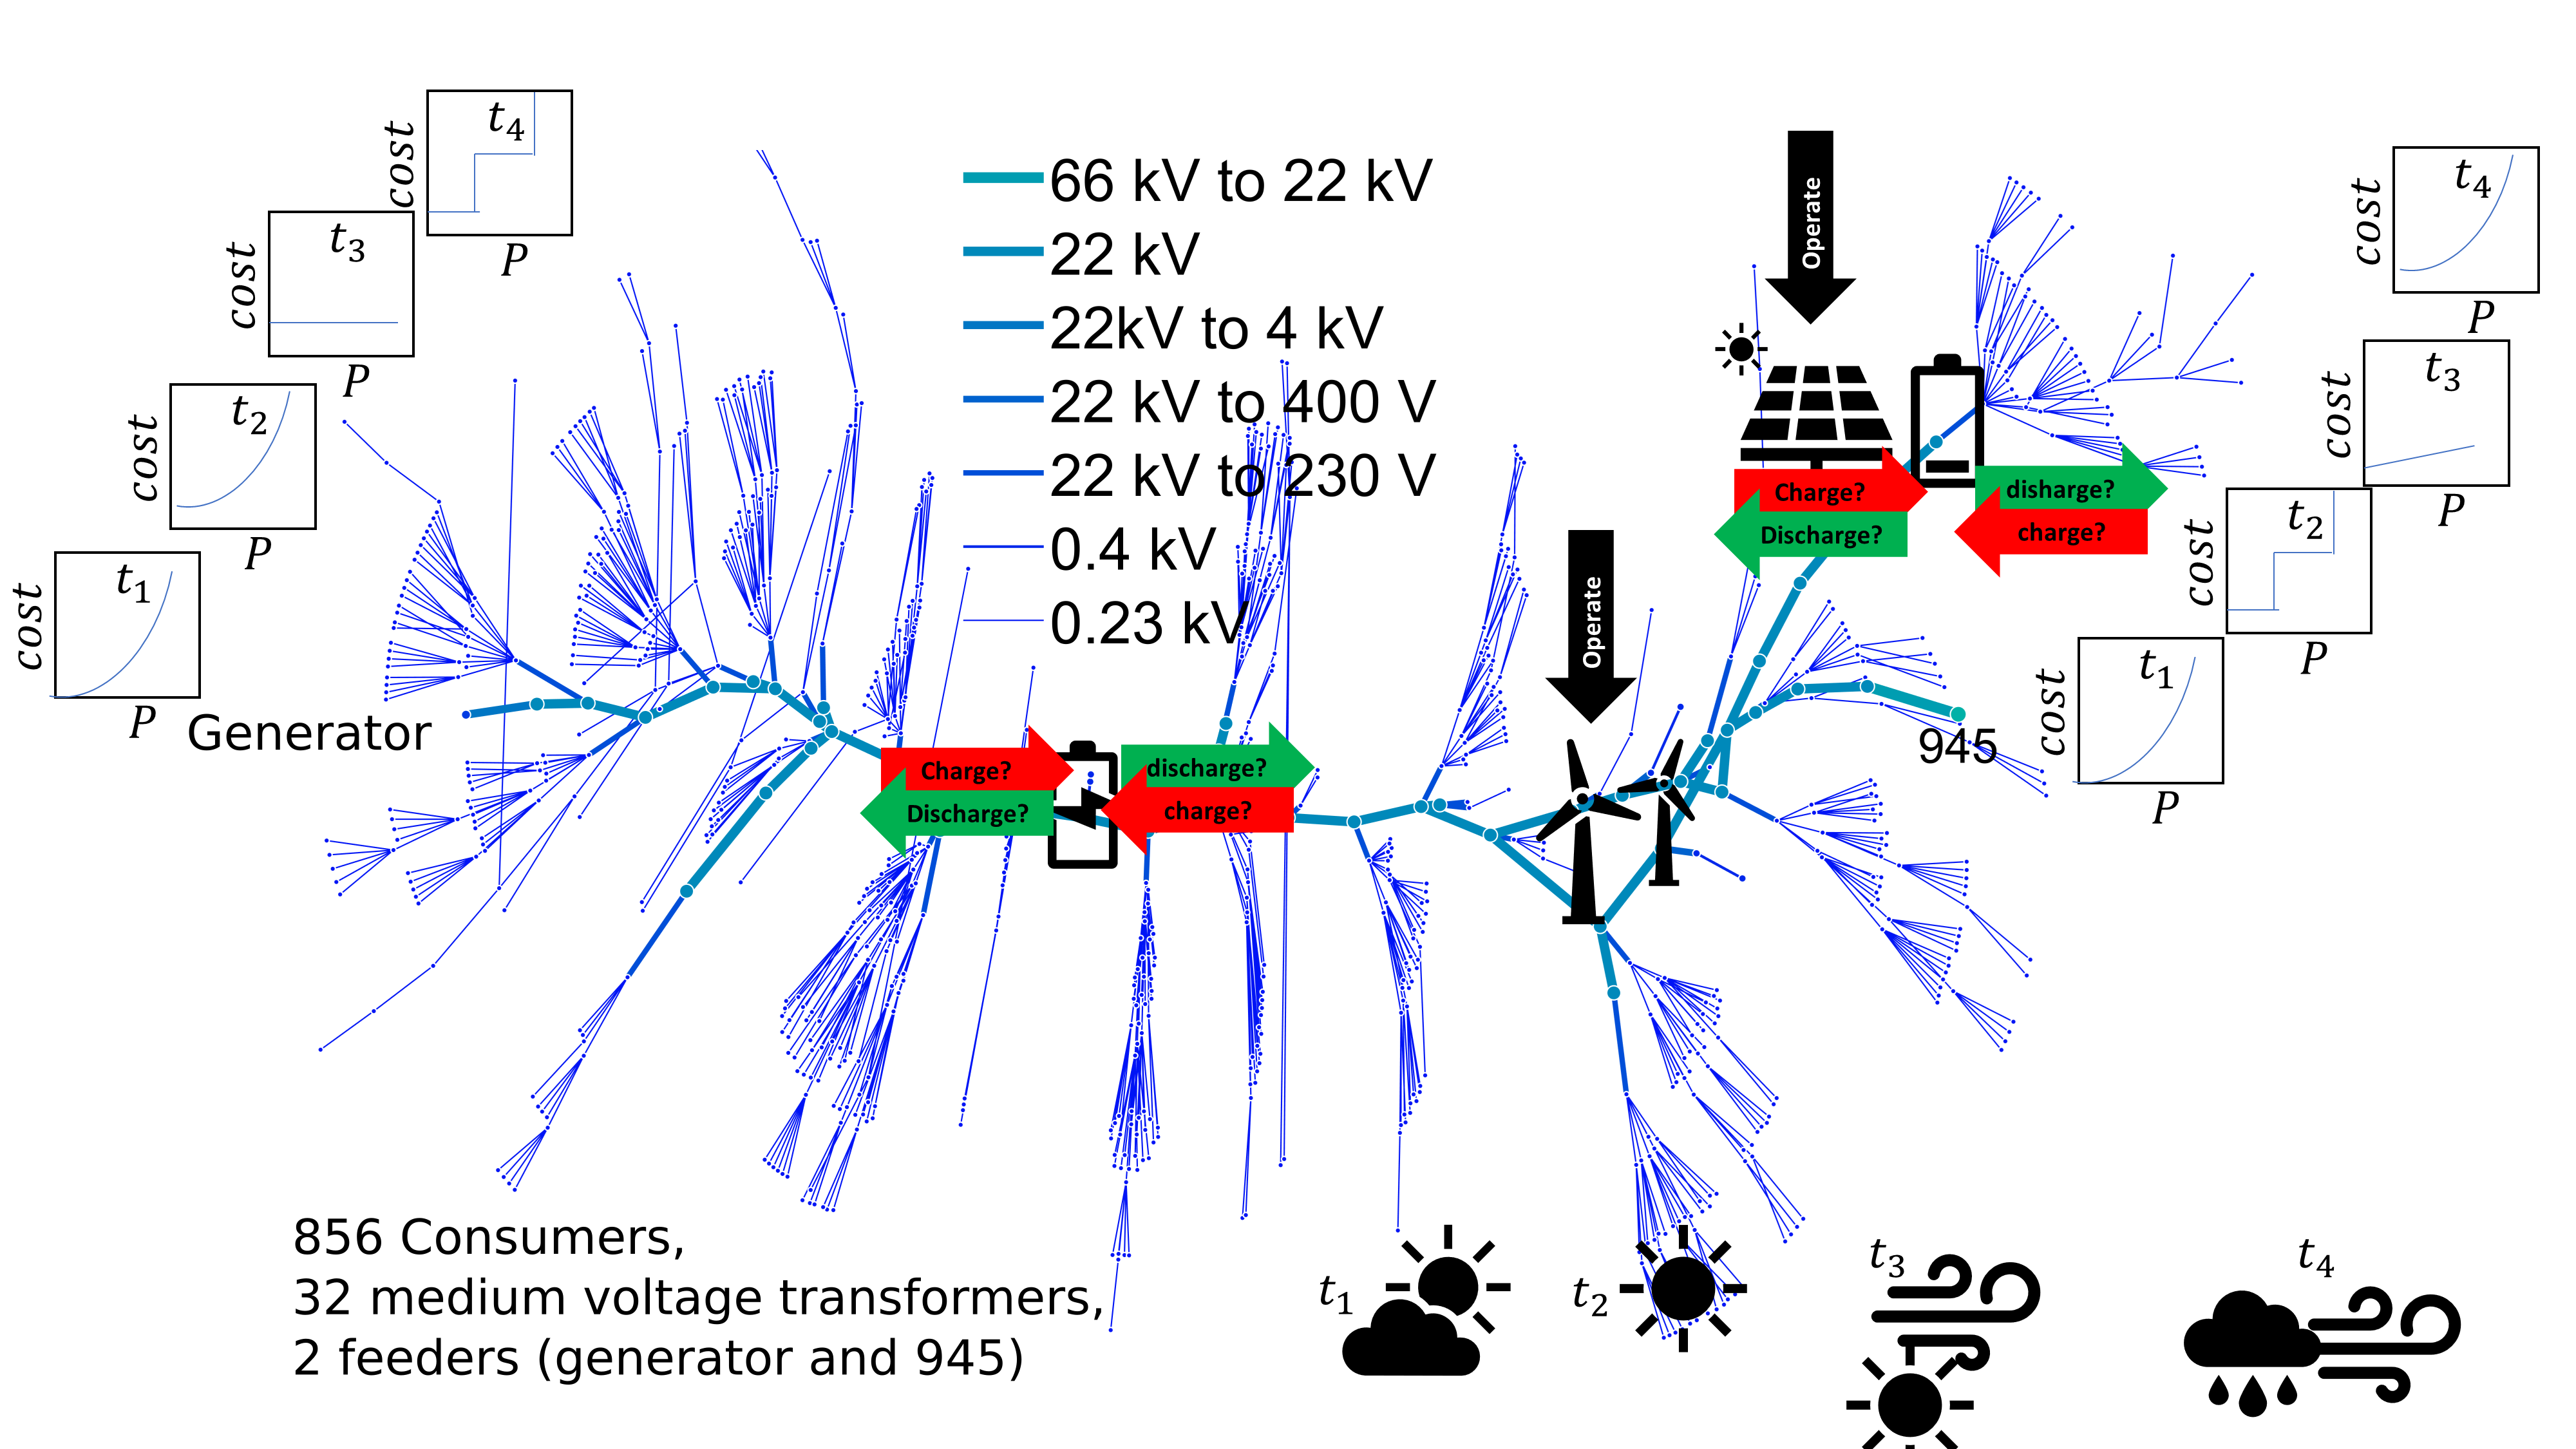
\includegraphics[width=3.5 in , height=2 in]{Figures/Presentation2/Slide3.png}
\caption{Local distribution grid located in Norway with 856 costumers}
\label{Norwegian1}
\end{figure}}
\only<8>{
\begin{figure}[!htbp]
\centering
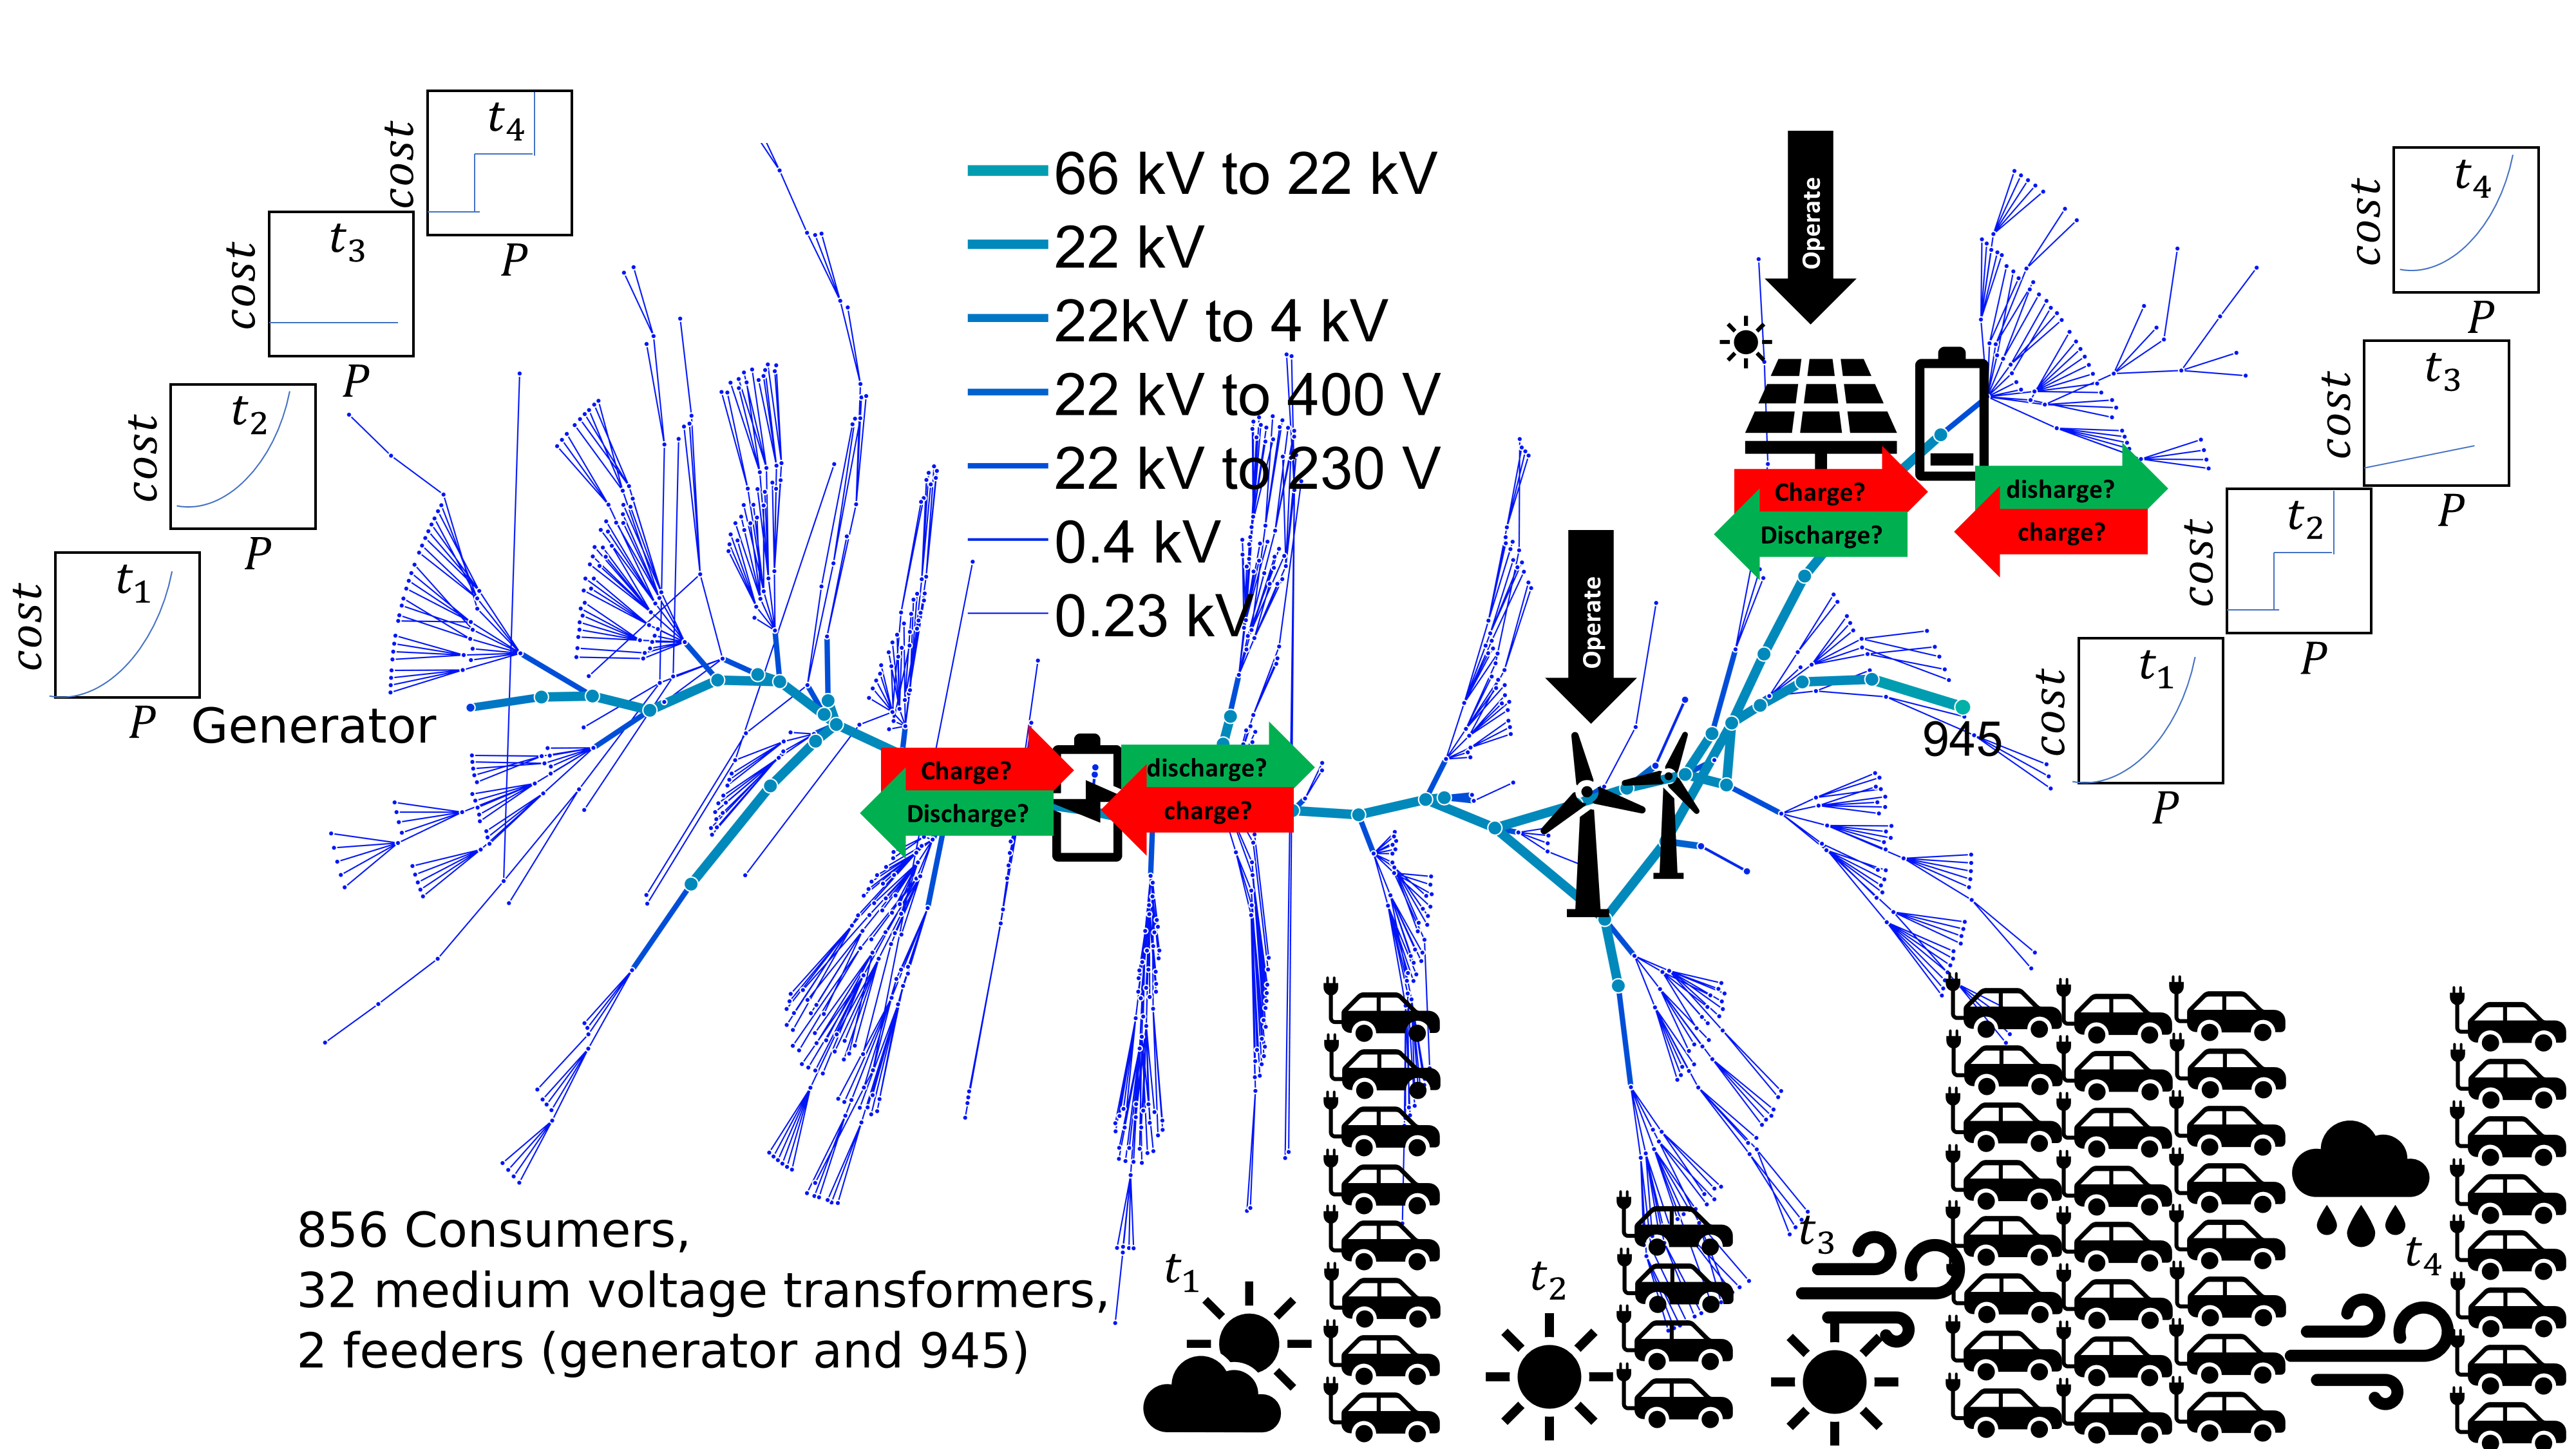
\includegraphics[width=3.5 in , height=2 in]{Figures/Presentation2/Slide4.png}
\caption{Local distribution grid located in Norway with 856 costumers}
\label{Norwegian1}
\end{figure}}
    \column{0.15\textwidth}
        \begin{figure}        
        
        
\includegraphics[scale=0.05]{Figures/IDEA.PNG}
        \end{figure}
\end{columns}
\end{frame}
%%%%%%%%%%%%%%%%%%%%%%%%%%%%%%%%%%%%%%%%%%
%%%%%%%%%%%%%%%%%%%%%%%%%%%%%%%%%%%%%%%%%%
%%%%%%%%%%%%%%%%%%%%%%%%%%%%%%%%%%%%%%%%%%
%%%%%%%%%%%%%%%%%%%%%%%%%%%%%%%%%%%%%%%%%%
\section{Papers}
\begin{frame}{Papers}
\centering \begin{block}{}
\begin{itemize}
\item<1-> \textbf{Paper I:} {\tiny Zaferanlouei, S., Farahmand, H., Vadlamudi, V. V., \& Korpas, M. (2021).} BATTPOWER Toolbox: Memory-Efficient and High-Performance MultiPeriod AC Optimal Power Flow Solver. IEEE Transactions on Power Systems.
\item<2-> \textbf{Paper II:} {\tiny Zaferanlouei, S., Lakshmanan, V., Bjarghov, S., Farahmand, H., \& Korpås, M. (2021).} BATTPOWER Application: Large-Scale Integration of EVs in an Active Distribution Grid--A Norwegian Case Study. arXiv preprint arXiv:2102.02677.
\end{itemize}
\end{block} 
\end{frame}
%%%%%%%%%%%%%%%%%%%%%%%%%%%%%%%%%%%%%%%%%%
%%%%%%%%%%%%%%%%%%%%%%%%%%%%%%%%%%%%%%%%%%
%%%%%%%%%%%%%%%%%%%%%%%%%%%%%%%%%%%%%%%%%%
%%%%%%%%%%%%%%%%%%%%%%%%%%%%%%%%%%%%%%%%%%
\section{Path}
\begin{frame}{Path from Research to Innovation}
\begin{backgroundblock}{20mm}{45mm}
    \begin{tikzpicture}
    \node[anchor=south west,inner sep=0] (B) at (4,0) {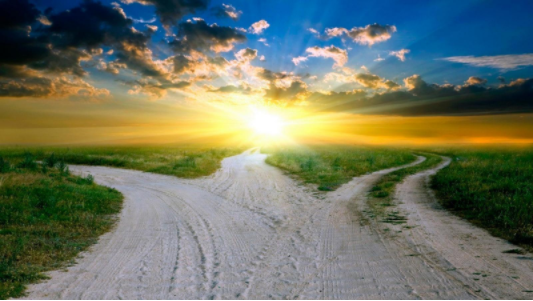
\includegraphics[width=\linewidth]{{Figures/Path.PNG}}};
        \fill [draw=none, fill=white, fill opacity=0.7] (B.north west) -- (B.north east) -- (B.south east) -- (B.south west) -- (B.north west) -- cycle;
    
    \end{tikzpicture} 
    \end{backgroundblock}    
{\scriptsize
\begin{block}{Path}
\begin{itemize}
\item<1-> I sent the "Disclosure of Innovation"  (DOFI) form to Technology Transfer Office (TTO)
\item<2-> Meeting with Technology Transfer Office (TTO)
\item<3-> Innovation Stipend Application
\item<4-> Meetings with Agder Energi, Norgesnett and Volue.
\item<5-> Discovery Project.
\end{itemize}
\end{block}}
\onslide<4> \begin{columns}
    \column{0.33\textwidth}
    
\includegraphics[scale=0.35]{Figures/Agder.png}
    \column{0.33\textwidth}
    
\includegraphics[scale=0.1]{Figures/Nett.jpg}
    \column{0.33\textwidth}
    
\includegraphics[scale=0.35]{Figures/Volue.jpg}
    \end{columns}
\end{frame}
%%%%%%%%%%%%%%%%%%%%%%%%%%%%%%%%%%%%%%%%%%
%%%%%%%%%%%%%%%%%%%%%%%%%%%%%%%%%%%%%%%%%%
%%%%%%%%%%%%%%%%%%%%%%%%%%%%%%%%%%%%%%%%%%
%%%%%%%%%%%%%%%%%%%%%%%%%%%%%%%%%%%%%%%%%%

\subsection{Send a DOFI}
\begin{frame}{DOFI is submitted on 27-08-2019}


\begin{backgroundblock}{30mm}{15mm}
    \begin{tikzpicture}
    \node[anchor=south west,inner sep=0] (B) at (4,0) {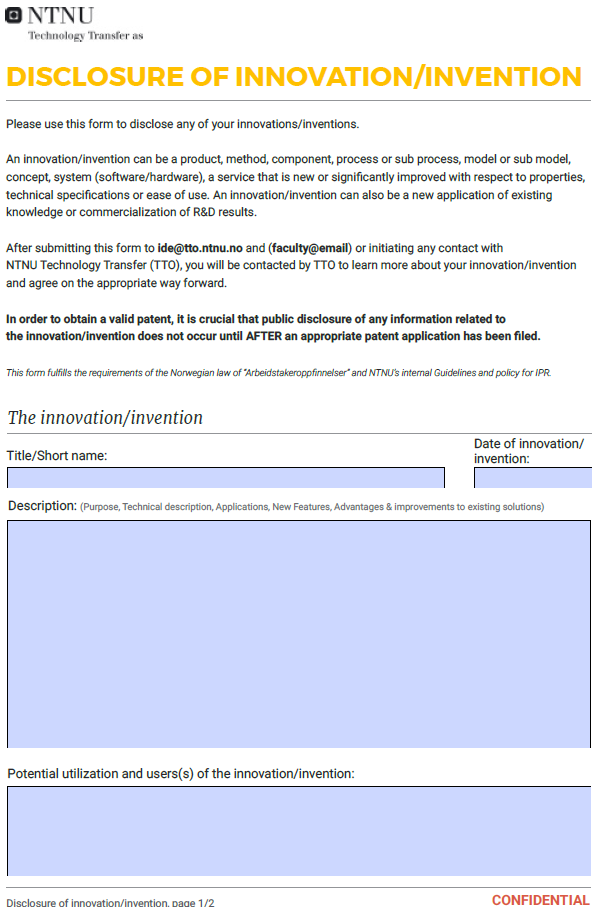
\includegraphics[width=\linewidth]{{Figures/DOFI.PNG}}};
        \fill [draw=none, fill=white, fill opacity=0.7] (B.north west) -- (B.north east) -- (B.south east) -- (B.south west) -- (B.north west) -- cycle;
    
    \end{tikzpicture}        
        
\end{backgroundblock}    

\begin{block}{Checklist}
\begin{enumerate}[I]
\item Title of your idea
\item Short description of Idea
\item Potential Market
\item What is the current stage of you idea? [a. Concept b. Preliminary c.Tested in practice d. Prototype]
\end{enumerate}
\end{block}    
    


\end{frame}
%%%%%%%%%%%%%%%%%%%%%%%%%%%%%%%%%%%%%%%%%%
%%%%%%%%%%%%%%%%%%%%%%%%%%%%%%%%%%%%%%%%%%
%%%%%%%%%%%%%%%%%%%%%%%%%%%%%%%%%%%%%%%%%%
%%%%%%%%%%%%%%%%%%%%%%%%%%%%%%%%%%%%%%%%%%
\subsection{Meeting with TTO}
\begin{frame}{First Meeting with TTO: Sep 2019}
\begin{alertblock}{\textcolor{red}{Everything started from here:}}
The core Battpower idea is presented for TTO.
\end{alertblock}

\begin{backgroundblock}{20mm}{30mm}
    \begin{tikzpicture}
    \node[anchor=south west,inner sep=0] (B) at (4,0) {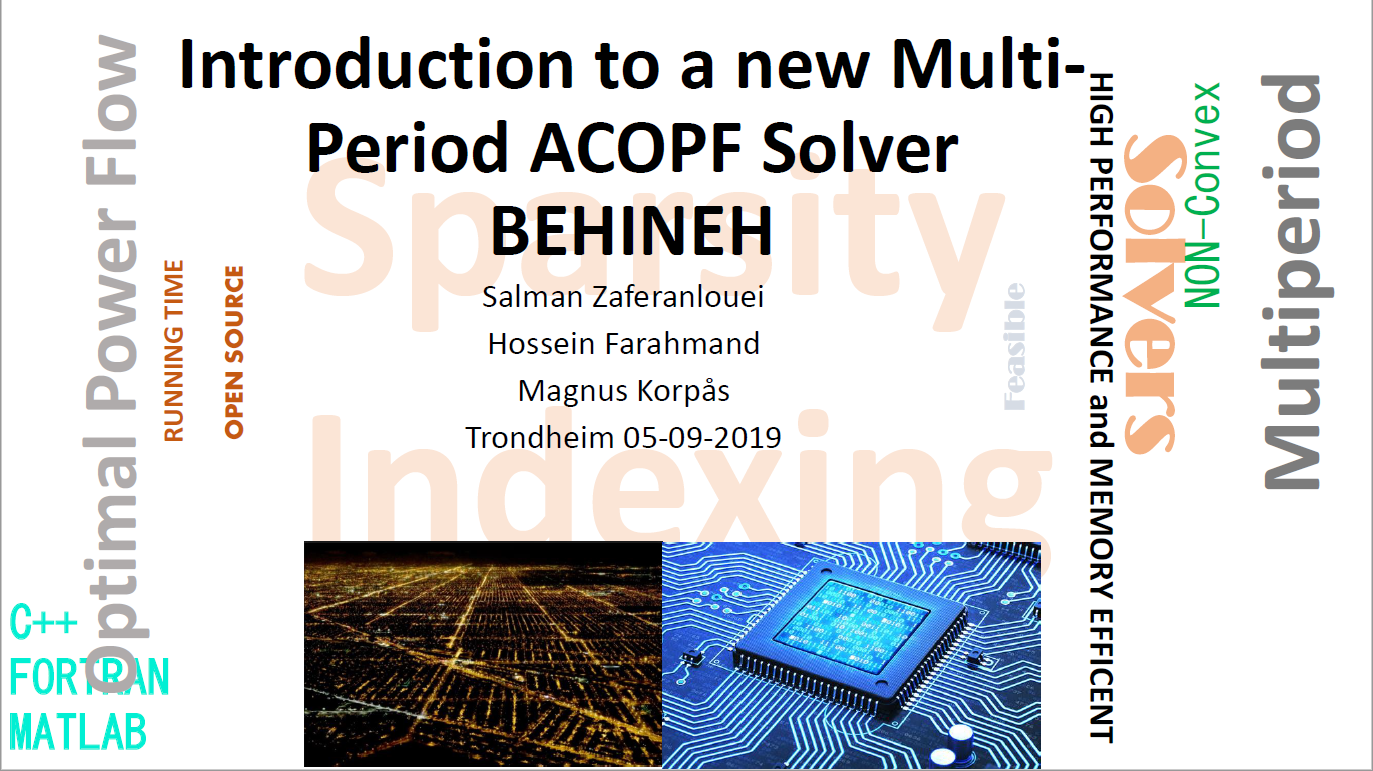
\includegraphics[width=\linewidth]{{Figures/FirstTTOMeeting.PNG}}};
        \fill [draw=none, fill=white, fill opacity=0.7] (B.north west) -- (B.north east) -- (B.south east) -- (B.south west) -- (B.north west) -- cycle;
    
    \end{tikzpicture}        
\end{backgroundblock} 


\end{frame}
%%%%%%%%%%%%%%%%%%%%%%%%%%%%%%%%%%%%%%%%%%
%%%%%%%%%%%%%%%%%%%%%%%%%%%%%%%%%%%%%%%%%%
%%%%%%%%%%%%%%%%%%%%%%%%%%%%%%%%%%%%%%%%%%
%%%%%%%%%%%%%%%%%%%%%%%%%%%%%%%%%%%%%%%%%%
\subsection{Innovasjonsstipend}
\begin{frame}{Innovation Grant (Innovasjonsstipend)}
\begin{backgroundblock}{20mm}{30mm}
    \begin{tikzpicture}
    \node[anchor=south west,inner sep=0] (B) at (4,0) {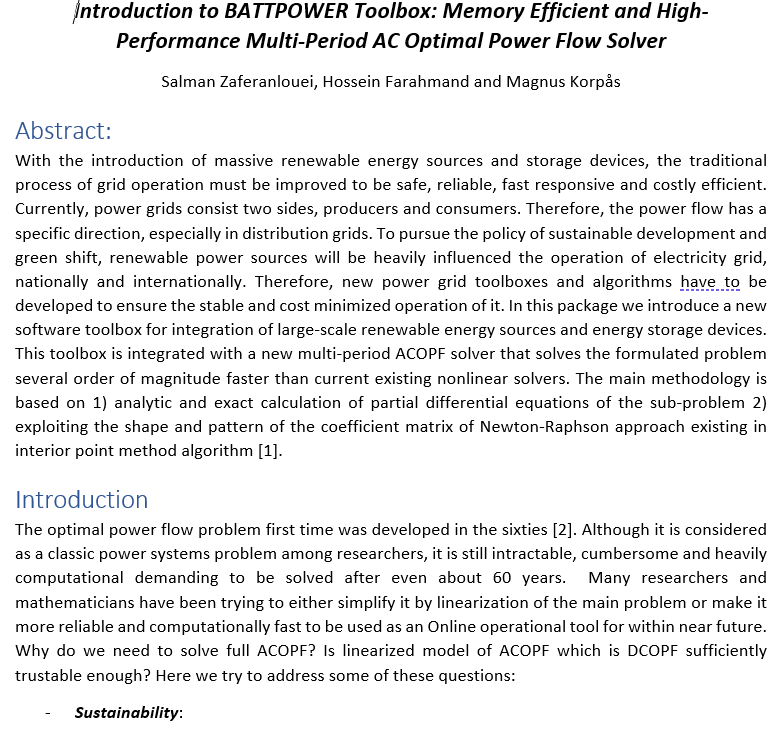
\includegraphics[width=\linewidth]{{Figures/Innovasjonsstipend.PNG}}};
        \fill [draw=none, fill=white, fill opacity=0.7] (B.north west) -- (B.north east) -- (B.south east) -- (B.south west) -- (B.north west) -- cycle;
    
    \end{tikzpicture}
\end{backgroundblock} 
\begin{alertblock}{\textcolor{red}{Milestones}}
\begin{itemize}
\item<1-> aim to release a preliminary version of the prototype solver in near future
\item<2-> benchmark the work with state of art commercial and open source solvers such as KNITRO, CONOPT and IPOPT
\item<3-> Apply for more funding
\end{itemize}
\end{alertblock}

\end{frame}
%%%%%%%%%%%%%%%%%%%%%%%%%%%%%%%%%%%%%%%%%%
%%%%%%%%%%%%%%%%%%%%%%%%%%%%%%%%%%%%%%%%%%
%%%%%%%%%%%%%%%%%%%%%%%%%%%%%%%%%%%%%%%%%%
%%%%%%%%%%%%%%%%%%%%%%%%%%%%%%%%%%%%%%%%%%
\subsection{Achievements of Innovasjonsstipend}
\begin{frame}{Innovasjonsstipend}
\begin{backgroundblock}{20mm}{30mm}
    \begin{tikzpicture}
    \node[anchor=south west,inner sep=0] (B) at (4,0) {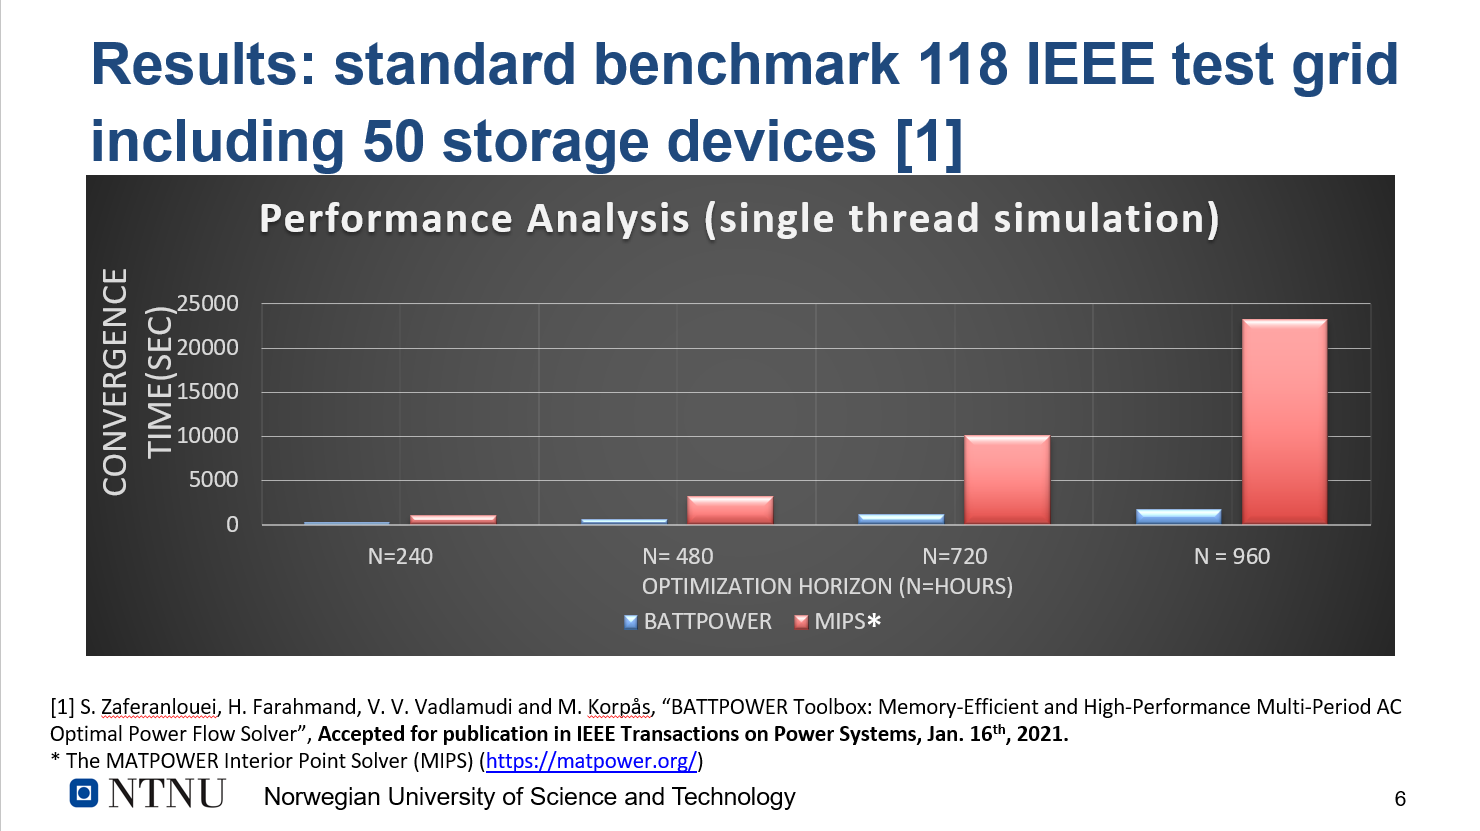
\includegraphics[width=\linewidth]{{Figures/Benchmark.PNG}}};
        \fill [draw=none, fill=white, fill opacity=0.7] (B.north west) -- (B.north east) -- (B.south east) -- (B.south west) -- (B.north west) -- cycle;
    
    \end{tikzpicture}
\end{backgroundblock} 
{\tiny
\begin{alertblock}{\textcolor{red}{Achievements}}

\begin{itemize}
\item<1-> Managed to get in contact with different companies: Agder Energi, Norgesnett and Volue.
\item<2-> We are currently collaborating with Volue.
\item<3-> Wrote an application for Radical Research Frontier (NFR application) \textcolor{blue}{\url{www.forskningsradet.no/en/call-for-proposals/2020/radical-frontier-research/}}
\item<4-> We are currently writing an \textcolor{red}{(Innovasjonsprosjekt  i  næringslivet) $\boldsymbol{IPN}$} application to build a partnership research collaboration between NTNU and Volue.
\item<5-> Applied for NTNU Discovery Project and managed to receive it 200,000 NOK. 
\end{itemize}
\end{alertblock}}
\onslide<1>{
\begin{columns}
    \column{0.33\textwidth}
    
\includegraphics[scale=0.35]{Figures/Agder.png}
    \column{0.33\textwidth}
    
\includegraphics[scale=0.1]{Figures/Nett.jpg}
    \column{0.33\textwidth}
    
\includegraphics[scale=0.35]{Figures/Volue.jpg}
    \end{columns}}
\onslide<2->{\centering
   
\includegraphics[scale=0.6]{Figures/Volue.jpg}}
\end{frame}

%%%%%%%%%%%%%%%%%%%%%%%%%%%%%%%%%%%%%%%%%%
%%%%%%%%%%%%%%%%%%%%%%%%%%%%%%%%%%%%%%%%%%
%%%%%%%%%%%%%%%%%%%%%%%%%%%%%%%%%%%%%%%%%%
%%%%%%%%%%%%%%%%%%%%%%%%%%%%%%%%%%%%%%%%%%
\subsection{Discovery Project}
\begin{frame}{Discovery Project}
\begin{block}{
We are now on this stage}
Discovery Project on board
\end{block}
\begin{alertblock}{Milestone}
\begin{itemize}
\item Move our codes to C++
\item Benchmark our final codes on a real distribution grid data.
\item Finalize the IPN proposal with Volue
\end{itemize}
\end{alertblock}
\end{frame}
%%%%%%%%%%%%%%%%%%%%%%%%%%%%%%%%%%%%%%%%%%
%%%%%%%%%%%%%%%%%%%%%%%%%%%%%%%%%%%%%%%%%%
%%%%%%%%%%%%%%%%%%%%%%%%%%%%%%%%%%%%%%%%%%
%%%%%%%%%%%%%%%%%%%%%%%%%%%%%%%%%%%%%%%%%%
\section{Opportunities}
\begin{frame}{Opportunities}
\begin{alertblock}{Opportunities}
\begin{itemize}
\item Through this process, (tto dis) excellent way to learn marketing and it is a different way than because you need to have hands on experience for it.
\item Things are different in real cases than research as there might be some details you have not taken into account before.
\end{itemize}
\end{alertblock}
\end{frame}


\begin{frame}{Different learning mechanism}
\onslide<1->\begin{block}{Learn a new subject}
I will explain this with an axample: imagine if you want to learn a Programming Language.
\end{block}

\only<1> {
        \begin{figure}
        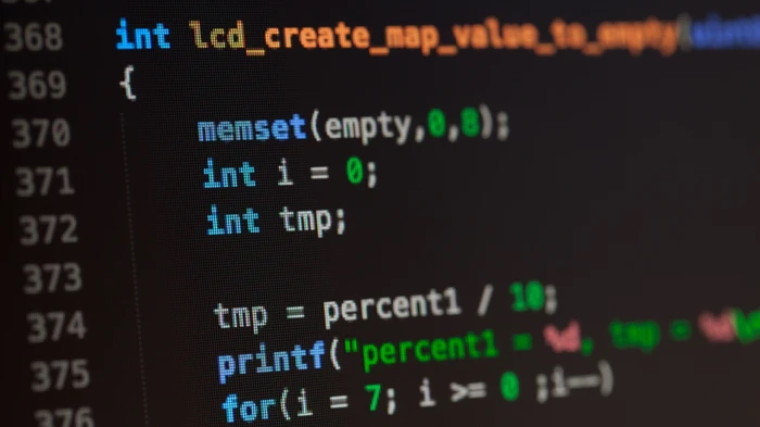
\includegraphics[scale=0.3]{Figures/CC.jpg}
        \end{figure}}

\onslide<2-> \begin{columns}
    \column{0.7\textwidth}
\begin{block}{Why do we use programming language?}
\begin{itemize}
\item<2-> To control machines:
\item<3-> To compute:
\item<4-> ... Many other applications
\end{itemize}
\end{block} 

    \column{0.3\textwidth}
    \only<2> {
        \begin{figure}
        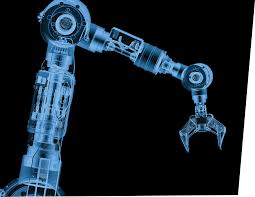
\includegraphics[scale=0.3]{Figures/MachineArm.jpg}
        \end{figure}}
        \only<3> {
        \begin{figure}
        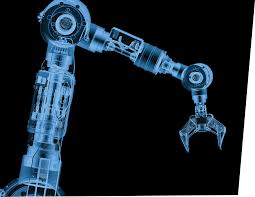
\includegraphics[scale=0.3]{Figures/MachineArm.jpg}
        \end{figure}
        \begin{figure}
        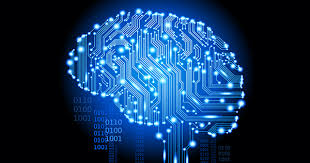
\includegraphics[scale=0.3]{Figures/Compute.jpg}
        \end{figure}}
                \only<4> {
        \begin{figure}
        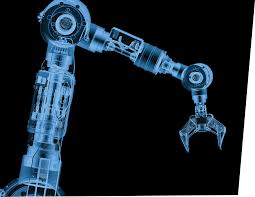
\includegraphics[scale=0.3]{Figures/MachineArm.jpg}
        \end{figure}
        \begin{figure}
        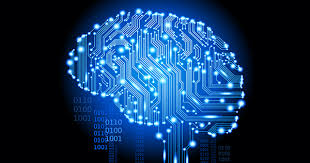
\includegraphics[scale=0.3]{Figures/Compute.jpg}
        \end{figure}}
\end{columns}
\end{frame}
%%%%%%%%%%%%%%%%%%%%%%%%%%%%%%%%%%%%%%%%%%
%%%%%%%%%%%%%%%%%%%%%%%%%%%%%%%%%%%%%%%%%%
%%%%%%%%%%%%%%%%%%%%%%%%%%%%%%%%%%%%%%%%%%
%%%%%%%%%%%%%%%%%%%%%%%%%%%%%%%%%%%%%%%%%%
\subsection{Innovation Route}
\begin{frame}{The challenges when you start to learn new things?}

\begin{block}{Challenges}

\begin{itemize}
\item<1-> Where to start?
\item<2-> What to do?
\end{itemize}
\end{block}
\end{frame}


\begin{frame}{Innovation route has also a similar route}
\begin{block}{Challenges}

\begin{itemize}
\item<1-> Where to start?
\item<2-> What to do?
\item<3-> How to do marketing?
\end{itemize}
\end{block}

\end{frame}
%%%%%%%%%%%%%%%%%%%%%%%%%%%%%%%%%%%%%%%%%%
%%%%%%%%%%%%%%%%%%%%%%%%%%%%%%%%%%%%%%%%%%
%%%%%%%%%%%%%%%%%%%%%%%%%%%%%%%%%%%%%%%%%%
%%%%%%%%%%%%%%%%%%%%%%%%%%%%%%%%%%%%%%%%%%
\begin{frame}{TTO}
\begin{block}{TTO helps you to learn this process!}
\begin{itemize}
\item<1-> Is the idea valuable?
\item<2-> Technology readiness level.
\item<3-> IPR.
\end{itemize}
\end{block}

\end{frame}
%%%%%%%%%%%%%%%%%%%%%%%%%%%%%%%%%%%%%%%%%%
%%%%%%%%%%%%%%%%%%%%%%%%%%%%%%%%%%%%%%%%%%
%%%%%%%%%%%%%%%%%%%%%%%%%%%%%%%%%%%%%%%%%%
%%%%%%%%%%%%%%%%%%%%%%%%%%%%%%%%%%%%%%%%%%
\section{Challenge}
\begin{frame}{Challenge}
\begin{alertblock}{secure funding}
\begin{itemize}
\item Apply for different calls.
\item You might end up without funding in between different projects grants. 
\end{itemize}

\end{alertblock}
\end{frame}
%%%%%%%%%%%%%%%%%%%%%%%%%%%%%%%%%%%%%%%%%%
%%%%%%%%%%%%%%%%%%%%%%%%%%%%%%%%%%%%%%%%%%
%%%%%%%%%%%%%%%%%%%%%%%%%%%%%%%%%%%%%%%%%%
%%%%%%%%%%%%%%%%%%%%%%%%%%%%%%%%%%%%%%%%%%
\begin{frame}
\centering
Any Question?\\
This presentation is recorded, therefore please contact me if you see this video later, and if you have any question: \textcolor{blue}{salman.zaf@ntnu.no}\\
\textcolor{blue}{\tiny \url{https://github.com/KavehZaf/NTNU_Presentations/tree/master/WebinarInnovation}}\\
Thank you for your attention!\\
		\vskip 0.8cm

\centering

\includegraphics[scale=0.2]{ntnulogo_eng.png}
\end{frame} 
%%%%%%%%%%%%%%%%%%%%%%%%%%%%%%%%%%%%%%%%%%
%%%%%%%%%%%%%%%%%%%%%%%%%%%%%%%%%%%%%%%%%%
%%%%%%%%%%%%%%%%%%%%%%%%%%%%%%%%%%%%%%%%%%
%%%%%%%%%%%%%%%%%%%%%%%%%%%%%%%%%%%%%%%%%%
\end{document}


